% !TEX program = pdflatex
\documentclass[aspectratio=169, 10pt]{beamer}

% ══════════════════════════════════════════════════════════════
%  TEMPLATE WHITELABEL — SISTEMAS RADAR
%  Edite apenas o bloco "DADOS DA APRESENTAÇÃO" abaixo.
%  Imagens necessárias na mesma pasta:
%    background_first.jpeg  (capa)
%    background.jpeg        (slides de seção)
%  Figuras: pasta figuras/ (geradas por gerar_graficos.py)
% ══════════════════════════════════════════════════════════════

% ── DADOS DA APRESENTAÇÃO ────────────────────────────────────
\newcommand{\apTitulo}{Aula 1 -- \texorpdfstring{\mbox{Revisão Teórica}}{Revisão Teórica}}
\newcommand{\apSubtitulo}{Sistemas Radar -- Curso de Especialização em Análise de Ambiente Eletromagnético}
\newcommand{\apAutores}{Arthur Cadore Matuella Barcella \enskip$\cdot$\enskip João Vitor Rosa Negri}
\newcommand{\apInstituicao}{Estágio de Docência -- Eng. Eletrônica e Computação (EEC-T)}
\newcommand{\apRodape}{SISTEMAS RADAR}      % texto à esquerda do rodapé
\newcommand{\apRodapeCentro}{Aula 1 -- Revisão teórica}   % texto central do rodapé
\newcommand{\apData}{\today}

% ── Tema base (minimal) ──────────────────────────────────────
\usetheme{default}
\setbeamertemplate{navigation symbols}{}
\setbeamertemplate{itemize item}{\scriptsize\raise1pt\hbox{\color{radarcyan}$\bullet$}}
\setbeamertemplate{itemize subitem}{\tiny\raise1pt\hbox{\color{radargreen}$\circ$}}
\setbeamertemplate{itemize subsubitem}{\tiny\raise1pt\hbox{\color{textsub}$-$}}

% ── Fontes modernas (Fira Sans) ──────────────────────────────
\usepackage[utf8]{inputenc}
\usepackage[T1]{fontenc}
\usepackage[sfdefault]{FiraSans}
\usepackage{FiraMono}

% ── Paleta de cores ──────────────────────────────────────────
\definecolor{bgdark}{RGB}{12,16,28}         % fundo principal
\definecolor{bgcard}{RGB}{20,28,50}         % fundo dos blocos
\definecolor{bglight}{RGB}{30,42,72}        % fundo mais claro para destaques
\definecolor{radarcyan}{RGB}{0,220,255}     % ciano radar — cor primária
\definecolor{radargreen}{RGB}{0,255,120}    % verde radar — acentos
\definecolor{accentblue}{RGB}{60,140,255}   % azul vibrante
\definecolor{alertred}{RGB}{255,80,80}      % vermelho para alertas
\definecolor{textmain}{RGB}{220,230,245}    % texto principal
\definecolor{textsub}{RGB}{140,160,200}     % texto secundário
\definecolor{accentgold}{RGB}{255,200,60}   % dourado para destaques

% ── Beamer: aplicar fundo escuro ─────────────────────────────
\setbeamercolor{background canvas}{bg=bgdark}
\setbeamercolor{normal text}{fg=textmain}
\setbeamercolor{structure}{fg=radarcyan}
\setbeamercolor{alerted text}{fg=alertred}
\setbeamercolor{example text}{fg=radargreen}

% Frametitle
\setbeamercolor{frametitle}{fg=white,bg=}
\setbeamerfont{frametitle}{size=\large, series=\bfseries}

% Itemize / enumerate
\setbeamercolor{itemize item}{fg=radarcyan}
\setbeamercolor{itemize subitem}{fg=radargreen}
\setbeamercolor{itemize subsubitem}{fg=textsub}
\setbeamercolor{enumerate item}{fg=radarcyan}

% Blocos
\setbeamercolor{block title}{fg=white,bg=accentblue!70!bgdark}
\setbeamercolor{block body}{fg=textmain,bg=bgcard}
\setbeamercolor{block title alerted}{fg=white,bg=alertred!80!bgdark}
\setbeamercolor{block body alerted}{fg=textmain,bg=alertred!8!bgdark}
\setbeamercolor{block title example}{fg=white,bg=radargreen!50!bgdark}
\setbeamercolor{block body example}{fg=textmain,bg=radargreen!5!bgdark}

% Tabelas — booktabs
\setbeamercolor{separation line}{bg=radarcyan!40}

% ── Frametitle com barra decorativa ──────────────────────────
\setbeamertemplate{frametitle}{%
  \nointerlineskip%
  \vskip8pt%
  \begin{beamercolorbox}[wd=\textwidth,leftskip=0.2cm]{frametitle}%
    {\usebeamerfont{frametitle}\usebeamercolor[fg]{frametitle}\insertframetitle}%
    \vskip2pt%
    \leavevmode%
    \begin{tikzpicture}
      \shade[left color=radarcyan, right color=bgdark, opacity=0.8] (0,0) rectangle (\textwidth-0.4cm, 0.035);
    \end{tikzpicture}%
  \end{beamercolorbox}%
}

% ── Footline com barra de progresso ──────────────────────────
\setbeamertemplate{footline}{%
  \begin{tikzpicture}[remember picture, overlay]
    \fill[bglight] (0,0) rectangle (\paperwidth, 0.35cm);
    \ifnum\inserttotalframenumber>0
      \pgfmathsetmacro{\progress}{\insertframenumber/\inserttotalframenumber}
      \shade[left color=radarcyan, right color=accentblue]
        (0,0) rectangle (\progress*\paperwidth, 0.35cm);
    \fi
    \node[anchor=west, font=\tiny\bfseries, text=textmain] at (0.15cm, 0.175cm)
      {\apRodape};
    \node[anchor=east, font=\tiny, text=textsub] at (\paperwidth-0.15cm, 0.175cm)
      {\insertframenumber\,/\,\inserttotalframenumber};
    \node[anchor=center, font=\tiny, text=textsub] at (0.5*\paperwidth, 0.175cm)
      {\apRodapeCentro};
  \end{tikzpicture}%
}

% ── Headline vazia ───────────────────────────────────────────
\setbeamertemplate{headline}{}

% ── Seção: slide de transição temático ───────────────────────
\AtBeginSection[]{%
  \begin{frame}[plain,noframenumbering]
    \begin{tikzpicture}[remember picture, overlay]
      % Imagem de fundo cobrindo o slide inteiro
      \node[anchor=center, inner sep=0pt] at (current page.center) {
        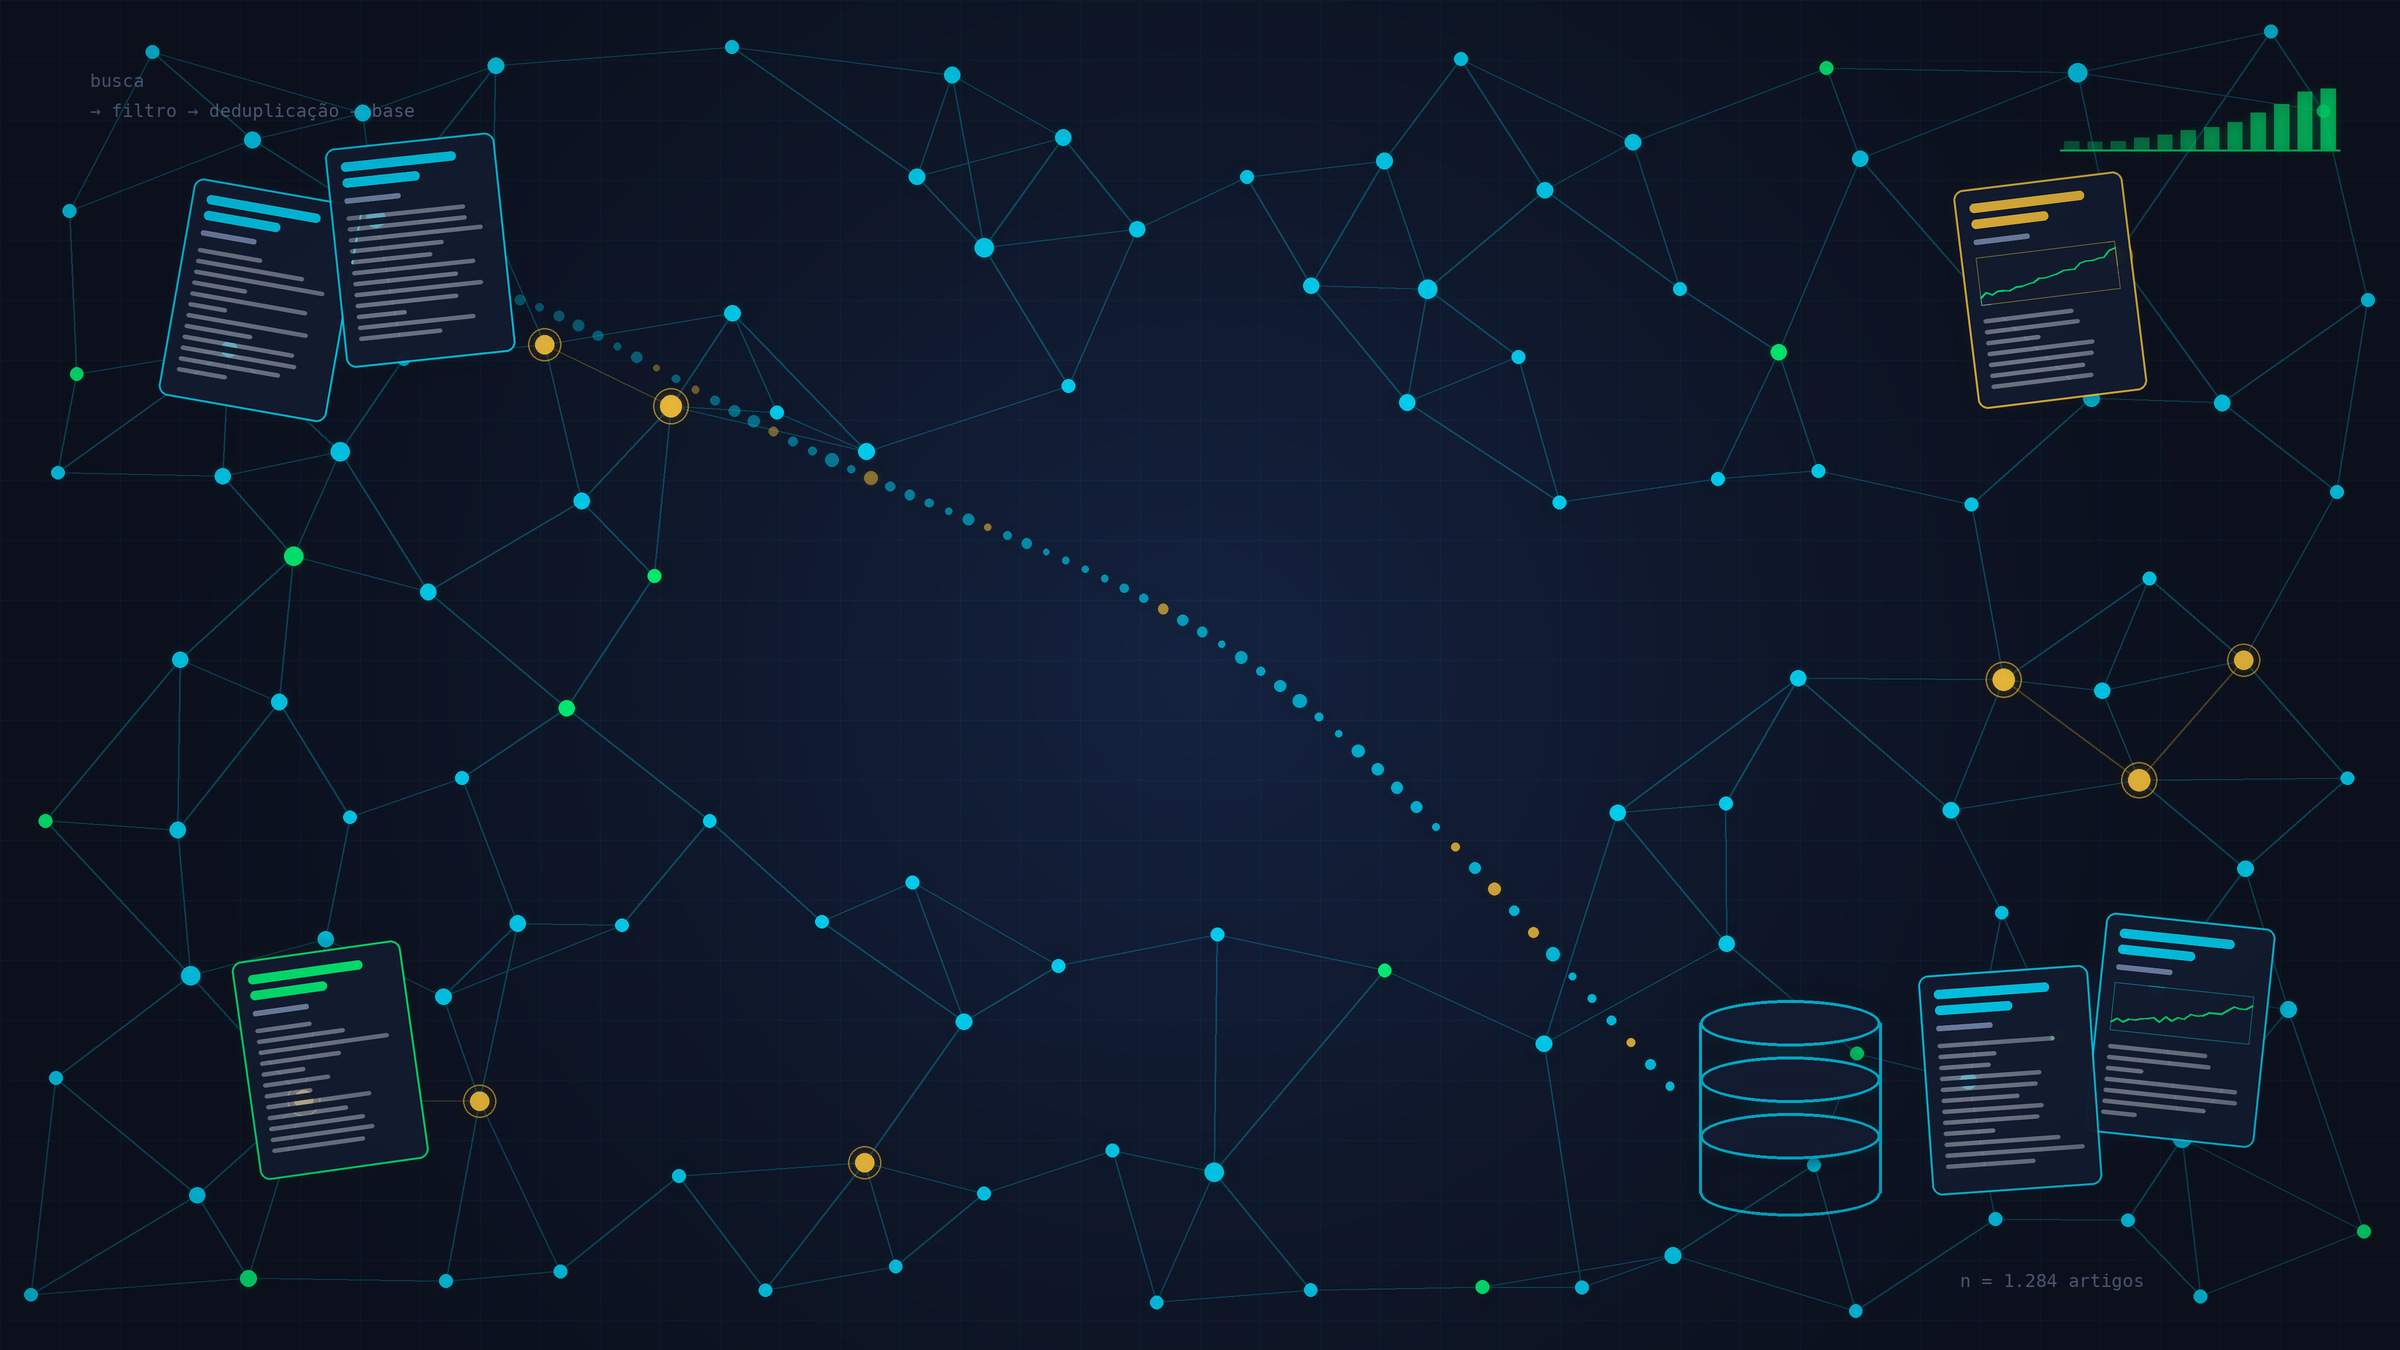
\includegraphics[width=\paperwidth, height=\paperheight]{background.jpeg}
      };
      % Overlay escuro para contraste
      \fill[bgdark, opacity=0.60] (current page.south west) rectangle (current page.north east);

      % Grid radar sutil
      \foreach \r in {1.2,2.4,...,6.0} {
        \draw[radarcyan!20, thin] (current page.center) circle (\r cm);
      }
      \draw[radarcyan!25, thin] (current page.center) -- ++(35:7.5cm);
      \draw[radarcyan!25, thin] (current page.center) -- ++(145:7.5cm);
      \draw[radarcyan!25, thin] (current page.center) -- ++(270:7.5cm);

      % Sweep sutil
      \fill[radarcyan, opacity=0.08] (current page.center) -- ++(55:7.5cm) arc (55:90:7.5cm) -- cycle;

      % Caixa com o título da seção
      \node[font=\LARGE\bfseries, text=white, fill=bgdark, fill opacity=0.88, text opacity=1, inner sep=12pt, rounded corners=8pt, draw=radarcyan!70, line width=1pt, align=center]
        at ([yshift=0.1cm]current page.center) {\insertsectionhead};
    \end{tikzpicture}
  \end{frame}
}

% ── Pacotes ───────────────────────────────────────────────────
\usepackage[brazil]{babel}
\usepackage{amsmath, amssymb, bm}
\usepackage{graphicx}
\usepackage{booktabs}
\usepackage{colortbl}
\usepackage{tikz}
\usetikzlibrary{arrows.meta, positioning, shapes.geometric, calc, decorations.pathreplacing, fadings}
\usepackage{listings}
\usepackage{hyperref}
\usepackage{caption}

% ── Estilos TikZ globais para fluxogramas ────────────────────
\tikzset{
  radarbox/.style={draw=#1!80, rounded corners, fill=#1!15!bgdark, minimum width=2.8cm, minimum height=0.65cm, font=\scriptsize, align=center, text=textmain},
  radarsmallbox/.style={draw=#1!80, rounded corners, fill=#1!15!bgdark, minimum width=1.9cm, minimum height=0.55cm, font=\scriptsize, align=center, text=textmain},
  radarmedbox/.style={draw=#1!80, rounded corners, fill=#1!15!bgdark, minimum width=2.4cm, minimum height=0.55cm, font=\scriptsize, align=center, text=textmain},
  radararr/.style={-{Stealth[length=2mm]}, thick, radarcyan!60}
}

\arrayrulecolor{radarcyan!40}

% ── Configuração de listings ─────────────────────────────────
\lstset{
  language=Python,
  basicstyle=\tiny\ttfamily\color{textmain},
  keywordstyle=\color{radarcyan}\bfseries,
  commentstyle=\color{textsub}\itshape,
  stringstyle=\color{radargreen},
  backgroundcolor=\color{bgcard},
  frame=single,
  rulecolor=\color{radarcyan!30},
  breaklines=true,
  columns=fullflexible,
}

% ── Macros auxiliares (reutilizáveis) ────────────────────────
\DeclareMathOperator{\sen}{sen}
% Moldura para figuras/gráficos (fundo branco sobre o tema escuro)
\newcommand{\plotbox}[2]{%
  \tikz\node[draw=radarcyan!45, line width=0.6pt, rounded corners=3pt, fill=white, inner sep=2pt]{\includegraphics[#1]{#2}};%
}
% Painel de equações
\newcommand{\eqpanel}[1]{%
  \begin{tikzpicture}
    \node[fill=bgcard, draw=radarcyan!40, line width=0.6pt, rounded corners=4pt,
          text width=\textwidth-12pt, inner sep=6pt, align=left, font=\small]{#1};
  \end{tikzpicture}%
}
\newcommand{\eqnote}[1]{\text{\footnotesize\color{textsub}#1}}
\setbeamerfont{block title}{size=\footnotesize, series=\bfseries}
\newcommand{\destaque}[1]{\textcolor{accentgold}{\bm{#1}}}

% ── Macros de conteúdo (Aula 1) ──────────────────────────────
% Figuras geradas por gerar_graficos.py (pasta figuras/)
\newcommand{\fig}[2][width=\dimexpr\linewidth-6pt\relax]{\plotbox{#1}{figuras/#2}}
% Rótulos coloridos
\newcommand{\rot}[2]{\textbf{\textcolor{#1}{#2}}}
\newcommand{\motiv}{\rot{accentgold}{Motivação:}\ }
\newcommand{\civil}{\rot{radargreen}{Civil:}\ }
\newcommand{\militar}{\rot{radarcyan}{Militar:}\ }
\newcommand{\ex}{\rot{accentgold}{Ex.:}\ }
% Informação que depende do laboratório e precisa ser confirmada/preenchida
\newcommand{\pendente}[1]{\textcolor{accentgold}{[\,#1\,]}}
% Unidades
\newcommand{\un}[1]{\,\mathrm{#1}}
\newcommand{\mus}{\,\mu\mathrm{s}}
\newcommand{\sinc}{\operatorname{sinc}}
% O painel de equações do modelo ocupa a largura toda; forçá-lo a ser um parágrafo
% próprio evita uma linha em branco quando ele é seguido de \vspace ou de uma lista.
\let\eqpanelmodelo\eqpanel
\renewcommand{\eqpanel}[1]{\par\eqpanelmodelo{#1}\par}
% Equação centralizada dentro de \eqpanel
\newcommand{\eqc}[1]{{\centering$\displaystyle #1$\par}}
% Blocos padronizados
\newenvironment{usos}{\begin{exampleblock}{Onde se usa}\footnotesize}{\end{exampleblock}}
\newenvironment{motivacao}{\begin{block}{Motivação}\footnotesize}{\end{block}}
% Tabelas
\newcolumntype{L}[1]{>{\raggedright\arraybackslash}p{#1}}
\newcommand{\cab}[1]{\textbf{\textcolor{radarcyan}{#1}}}
% Aproveita melhor a altura útil: reduz o espaço entre a barra do título e o conteúdo
\addtobeamertemplate{frametitle}{}{\vspace{-6pt}}
\setlength{\leftmargini}{1.1em}
\setlength{\leftmarginii}{1.0em}

% ── Metadados ─────────────────────────────────────────────────
\title[\apTitulo]{\apTitulo\\ \small \apSubtitulo}
\author{\apAutores}
\date{\apData}

% ══════════════════════════════════════════════════════════════
\begin{document}

% ── Capa ──────────────────────────────────────────────────────
\begin{frame}[plain,noframenumbering]
  \begin{tikzpicture}[remember picture, overlay]
    \fill[bgdark] (current page.south west) rectangle (current page.north east);
    \node[anchor=east, inner sep=0pt] at (current page.east) {
      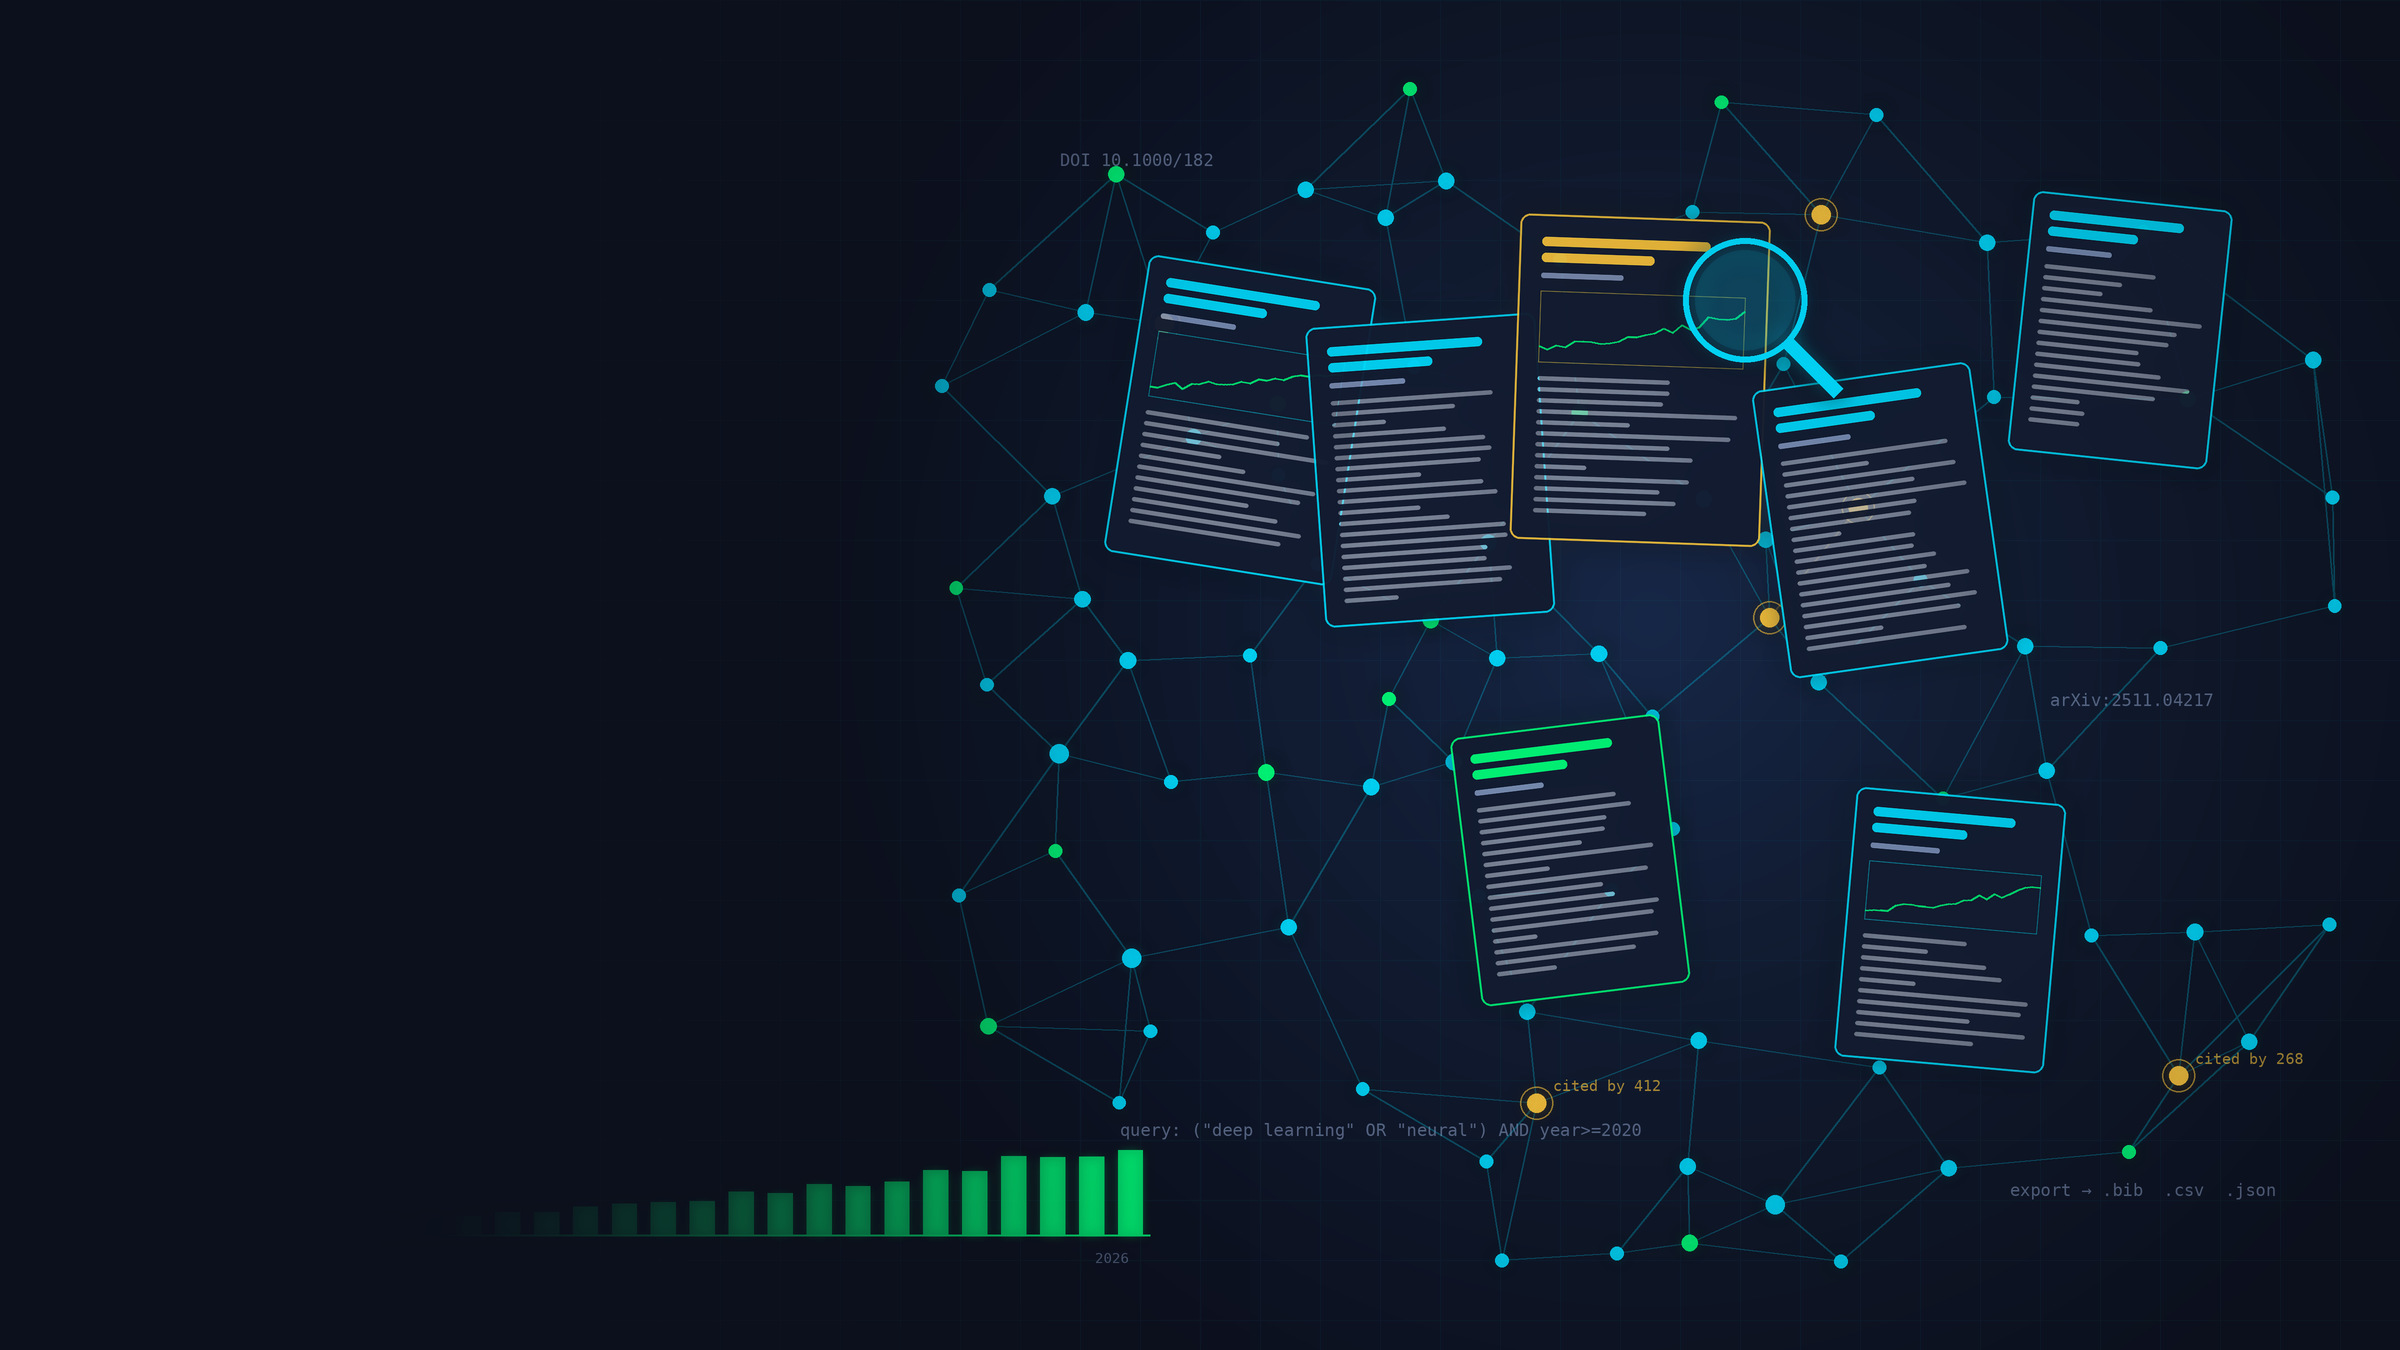
\includegraphics[height=\paperheight, keepaspectratio]{background_first.jpeg}
    };
    % (o degradê esquerdo da imagem já está embutido em background_first.jpeg)

    \shade[top color=radarcyan, bottom color=radarcyan!5!bgdark, opacity=0.8]
      ([xshift=1.0cm, yshift=-0.8cm]current page.north west) rectangle ++(0.08cm,-6.8cm);

    \node[anchor=south west, font=\fontsize{22}{27}\selectfont\bfseries, text=white, text width=8.5cm, align=left]
      at ([xshift=1.5cm, yshift=1.15cm]current page.west) {\apTitulo};

    \node[anchor=west, font=\small, text=textsub, text width=8.5cm, align=left]
      at ([xshift=1.5cm, yshift=0.75cm]current page.west) {\apSubtitulo};

    \shade[left color=radarcyan, right color=radarcyan!5!bgdark]
      ([xshift=1.5cm, yshift=0.15cm]current page.west) rectangle ++(6.5cm,0.04cm);

    \node[anchor=west, font=\footnotesize, text=radarcyan, text width=8.5cm, align=left]
      at ([xshift=1.5cm, yshift=-0.45cm]current page.west) {\apAutores};

    \node[anchor=west, font=\footnotesize, text=textsub, text width=8.5cm, align=left]
      at ([xshift=1.5cm, yshift=-1.05cm]current page.west) {\apInstituicao};

    \node[anchor=west, font=\scriptsize, text=textsub!70, text width=8.5cm, align=left]
      at ([xshift=1.5cm, yshift=-1.55cm]current page.west) {\apData};

    \shade[left color=radarcyan!40, right color=accentblue!40]
      ([yshift=0.5cm]current page.south west) rectangle ([yshift=0.54cm]current page.south east);
  \end{tikzpicture}
\end{frame}

% ── Sumário ───────────────────────────────────────────────────
\begin{frame}[t]{Sumário}
  \small
  \begin{columns}[T,onlytextwidth]
    \begin{column}{0.48\textwidth}
      \tableofcontents[sections={1-6}]
    \end{column}
    \begin{column}{0.48\textwidth}
      \tableofcontents[sections={7-11}]
    \end{column}
  \end{columns}
\end{frame}

% ══════════════════════════════════════════════════════════════
\section{Objetivos}
% ══════════════════════════════════════════════════════════════


\begin{frame}[t]{Objetivos gerais}
  \small
  Ao final desta aula o aluno deve ser capaz de:
  \begin{itemize}\setlength{\itemsep}{1pt}
    \item Ler os parâmetros de um pulso de radar (PRI, PW, potência, modulação) e relacioná-los a alcance, resolução e função do radar.
    \item Explicar por que se usa modulação intrapulso e reconhecer LFM, PSK, FSK e FMCW.
    \item Relacionar frequência de operação e antena com a aplicação do radar.
    \item Entender ruído, clutter, limiar (threshold), histerese e CFAR no processo de detecção.
    \item Interpretar Doppler, atraso e amplitude do sinal recebido, e os conceitos de DOA e deinterleaving.
    % \item Conhecer o ambiente de simulação (Sim View, gerador, analisador/osciloscópio e VSA) usado nas próximas aulas.
  \end{itemize}
\end{frame}

% ══════════════════════════════════════════════════════════════
\section{Parâmetros de Sistemas Radar}
% ══════════════════════════════════════════════════════════════

\begin{frame}[t]{Parâmetros de pulso de radar}
  \begin{columns}[T,onlytextwidth]
    \begin{column}{0.36\textwidth}
      \footnotesize
      Um sistema radar pulsado é definido por alguns parâmetros principais:
      \begin{itemize}\setlength{\itemsep}{0pt}
        \item \textbf{PRI}, período de repetição do pulso. 
        \item \textbf{PW} largura de pulso, $\tau$
        \item \textbf{Potência} de pico e média
        \item \textbf{Frequência} da portadora $f_c$
        \item \textbf{Modulação} dentro do pulso
        \item \textbf{Varredura} da antena
      \end{itemize}
    \end{column}
    \begin{column}{0.62\textwidth}
      \fig{pulso_parametros}
    \end{column}
  \end{columns}
\end{frame}


\begin{frame}[t]{PRI -- Pulse Repetition Interval}
  \begin{columns}[T,onlytextwidth]
    \begin{column}{0.37\textwidth}
      \footnotesize
      Tempo entre o início de dois pulsos consecutivos.
      \vspace{3pt}

      \eqpanel{%
        \eqc{R_{max}=\frac{c\,PRI}{2}}
      }
      \vspace{3pt}
      \motiv PRI longa vê longe sem ambiguidade de distância, porem com menor energia média; PRI curta adiciona mais energia no alvo, mas diminuia a distância. 
    \end{column}
    \begin{column}{0.61\textwidth}
      \fig{pri_ambiguidade}
    \end{column}
  \end{columns}
\end{frame}

\begin{frame}[t]{PW -- Pulse Width}
  \begin{columns}[T,onlytextwidth]
    \begin{column}{0.37\textwidth}
      \footnotesize
      Duração do pulso transmitido ($\tau$).
      \vspace{3pt}

      \eqpanel{%
        \eqc{R_{min}=\frac{c\,\tau}{2}}
        \vspace{3pt}
        \eqc{E=P_p\,\tau\qquad B\approx\frac{1}{\tau}}
      }
      \vspace{3pt}
      \motiv Pulso longo possui mais energia e portanto maior alcance, e aumenta a zona cega ($R_{min}$); pulso curto tem melhor resolução e dimunui a zona cega ($R_{min}$). Esse conflito é o que a compressão de pulso resolve.
    \end{column}
    \begin{column}{0.61\textwidth}
      \fig{pw_resolucao}
    \end{column}
  \end{columns}
\end{frame}

\begin{frame}[t]{Relação entre PRI e PW}
  \begin{columns}[T,onlytextwidth]
    \begin{column}{0.36\textwidth}
      \footnotesize
      A relação entre a PRI e a PW define o ciclo de trabalho (duty cycle) do sistema.
      \vspace{3pt}
      \eqpanel{%
        \eqc{d=\frac{\tau}{PRI}}
        \vspace{3pt}
        \eqc{P_m=P_p\,d}
        \vspace{3pt}
        \eqc{\frac{c\,\tau}{2}\;<\;R\;<\;\frac{c\, PRI}{2}}
        }
        \vspace{3pt}
        \motiv Periodo de trabalho baixo (duty cycle) significa que o radar está transmitindo pouco tempo, e portanto com menor potência média; periodo de trabalho alto significa que o radar está transmitindo mais tempo, e portanto com maior potência média.
    \end{column}
    \begin{column}{0.62\textwidth}
      \footnotesize
      \renewcommand{\arraystretch}{1.05}
      \begin{tabular}{@{}L{2.75cm}L{1.5cm}L{1.85cm}L{1.25cm}@{}}
        \toprule
        \cab{Tipo de radar} & \cab{PW} & \cab{PRF} & \cab{Ciclo} \\
        \midrule
        Navegação marítima (magnetron) & 0,05--1\,$\mu$s & 0,5--3\,kHz & $<0{,}1$\,\% \\
        Vigilância aérea (válvula) & $\sim$1\,$\mu$s & 0,3--1,2\,kHz & $\sim$0,1\,\% \\
        Vigilância aérea (estado sólido) & 1--100\,$\mu$s & 0,3--1,2\,kHz & até $\sim$10\,\% \\
        Meteorológico & 1--5\,$\mu$s & 0,3--1,3\,kHz & 0,1--0,2\,\% \\
        Pulso-Doppler de caça (alta PRF) & $\sim$1\,$\mu$s & 100--300\,kHz & 10--50\,\% \\
        FMCW (altímetro, automotivo) & contínuo & --- & 100\,\% \\
        \bottomrule
      \end{tabular}

      {\scriptsize\color{textsub}Valores típicos, apenas ordem de grandeza.}
    \end{column}
  \end{columns}
\end{frame}

\begin{frame}[t]{Medição de distância a partir do sinal recebido}
  \begin{columns}[T,onlytextwidth]
    \begin{column}{0.36\textwidth}
      \footnotesize
      O radar mede o tempo entre a transmissão e a chegada do eco.
      \vspace{2pt}

      \eqpanel{%
        \eqc{R=\frac{c\,\Delta t}{2}}
        \vspace{3pt}
        \eqc{\delta R\approx\frac{c}{2B\sqrt{2\,\mathrm{SNR}}}}
        \vspace{1pt}}
      \vspace{2pt}

      \begin{itemize}\setlength{\itemsep}{0pt}
        \item 1\,$\mu$s equivale a 150\,m.
        \item 1\,km equivale a 6,67\,$\mu$s.
      \end{itemize}

      \motiv é a medida fundamental do radar, e exige conhecer o instante da transmissão. Um receptor passivo (RWR) não tem essa referência: vê o tempo de chegada, e não a distância.\\[1pt]
    \end{column}
    \begin{column}{0.62\textwidth}
      \fig{atraso_distancia}

    \end{column}
  \end{columns}
\end{frame}


% ══════════════════════════════════════════════════════════════
\section{Modulação intrapulso}
% ══════════════════════════════════════════════════════════════

\begin{frame}[t]{Problema do pulso simples}
  \begin{columns}[T,onlytextwidth]
    \begin{column}{0.37\textwidth}
      \footnotesize
      Quando temos dois alvos próximos, um radar com pulso simples não consegue resolver a ambiguidade de distância, pois o pulso transmitido é longo e a resolução é baixa.
      \vspace{2pt}

      \eqpanel{%
        \eqc{\Delta R=\frac{c}{2B}}
        \vspace{2pt}
        {\footnotesize\color{textsub}Vale para qualquer forma de onda. Pulso simples: $B\approx1/\tau$ $\Rightarrow$ $c\tau/2$.}}
      \vspace{3pt}

      \renewcommand{\arraystretch}{1.05}
      \begin{tabular}{@{}L{1.9cm}L{2.2cm}@{}}
        \toprule
        \cab{Banda} & \cab{$\Delta R$} \\
        \midrule
        1\,MHz & 150\,m \\
        5\,MHz & 30\,m \\
        150\,MHz & 1\,m \\
        1\,GHz & 15\,cm \\
        \bottomrule
      \end{tabular}
    \end{column}
    \begin{column}{0.61\textwidth}
      \fig{resolucao_alcance}

      \vspace{2pt}
      \footnotesize
      \motiv separar alvos próximos (exemplo: aeronaves em formação), em azul, sem modulação o radar não consegue distinguir os dois alvos, em laranja, com modulação intrapulso o radar consegue distinguir os dois alvos.
    \end{column}
  \end{columns}
\end{frame}

\begin{frame}[t]{Motivação da modulação intrapulso}
  \centering
  \begin{tikzpicture}[node distance=0.55cm]
    \node[radarbox=radarcyan, minimum width=2.9cm] (tx) {Pulso longo modulado\\ duração $\tau$, banda $B$};
    \node[radarbox=accentblue, right=of tx, minimum width=2.2cm] (alvo) {Propagação\\ e alvo};
    \node[radarbox=radargreen, right=of alvo, minimum width=2.5cm] (fc) {Filtro casado\\ (correlação)};
    \node[radarbox=accentgold, right=of fc, minimum width=2.9cm] (out) {Pulso comprimido\\ largura $\approx 1/B$};
    \draw[radararr] (tx) -- (alvo);
    \draw[radararr] (alvo) -- (fc);
    \draw[radararr] (fc) -- (out);
  \end{tikzpicture}
  \vspace{4pt}
  \begin{columns}[T,onlytextwidth]
    \begin{column}{0.37\textwidth}
      \footnotesize
      \rot{alertred}{Radar com pulso simples}
      \begin{itemize}\setlength{\itemsep}{0pt}
        \item Alcance pede energia, $E=P_p\,\tau$, logo $\tau$ grande.
        \item Resolução pede $\tau$ pequeno, $\Delta R=c\tau/2$.
        \item Aumentar $P_p$ tem limite de hardware (alta tensão, custo, etc).
      \end{itemize}
      \rot{radargreen}{Radar com pulso modulado}
      \begin{itemize}\setlength{\itemsep}{0pt}
        \item A SNR na saída do filtro casado só depende da energia: $\mathrm{SNR}=2E/N_0$.
        \item Mesma energia, mesmo pico; a largura passa a ser $1/B$.
      \end{itemize}
    \end{column}
    \begin{column}{0.61\textwidth}
      \fig{compressao_pulso}
      \vspace{2pt}
      \footnotesize
      Os dois pulsos têm a mesma duração e a mesma energia. Depois do filtro casado, o pulso com LFM fica 50 vezes mais estreito ($B\tau=50$).
    \end{column}
  \end{columns}
\end{frame}

\begin{frame}[t]{Revisando Filtro Casado}
  \begin{columns}[T,onlytextwidth]
    \begin{column}{0.37\textwidth}
      \footnotesize
      Um filtro casado relaciona o pulso recebido com o pulso transmitido, com o objetivo de correlacionar o sinal conhecido e descorrelacionar o ruído e interferências adicionadas ao sinal, otimizando a SNR do sinal. 
    \end{column}
    \begin{column}{0.61\textwidth}
      COLOCAR UMA IMAGEM DE SINAL DE TX, SINAL DE RX COM RUIDO E SAIDA DO FILTRO CASADO
    
    \end{column}
  \end{columns}
\end{frame}



\begin{frame}[t]{Tipos de modulação}
  \begin{columns}[T,onlytextwidth]
    \begin{column}{0.37\textwidth}
      \footnotesize
      \rot{radarcyan}{Dentro do pulso (intrapulso)}
      \begin{itemize}\setlength{\itemsep}{1pt}
        \item \textbf{Sem modulação}: portadora pura. 
        \item \textbf{Em frequência}: LFM (chirp), NLFM, FSK/Costas.
        \item \textbf{Em fase}: BPSK/Barker, polifásica, etc.
      \end{itemize}
      \rot{radarcyan}{Onda contínua (Radar \textbf{não} pulsado)}
      \begin{itemize}\setlength{\itemsep}{1pt}
        \item CW (só Doppler) e FMCW.
      \end{itemize}
      \vspace{2pt}
      {\footnotesize\motiv a modulação define banda, resolução e facilidade de interceptação. }
    \end{column}
    \begin{column}{0.61\textwidth}
      \fig{modulacoes_panorama}
    \end{column}
  \end{columns}
\end{frame}


\begin{frame}[t]{Banda ocupada pelo pulso}
  \begin{columns}[T,onlytextwidth]
    \begin{column}{0.50\textwidth}
      \footnotesize
      A banda depende da modulação, e não só da duração:
      \vspace{2pt}

      \renewcommand{\arraystretch}{1.15}
      \begin{tabular}{@{}L{2.5cm}L{3.9cm}@{}}
        \toprule
        \cab{Forma de onda} & \cab{Banda aproximada} \\
        \midrule
        Sem modulação & $B\approx 1/\tau$ \\
        LFM & $B\approx$ $\Delta f$ \\
        PSK & $B\approx 1/\tau_c$ (taxa de chips) \\
        FSK & $B\approx N\,\Delta f$ \\
        \bottomrule
      \end{tabular}
      \vspace{3pt}

      \begin{itemize}\setlength{\itemsep}{0pt}
        \item O ruído cresce com a banda ($N=kTB\,F$). 
        \item O filtro casado entrega ganho $B\tau$.
      \end{itemize}
      \motiv a banda é o ``preço'' da resolução. Quem projeta o radar escolhe $B$; quem analisa o sinal lê $B$ no espectro e deduz a resolução do radar.
    \end{column}
    \begin{column}{0.48\textwidth}
      \fig{banda_espectro}
    \end{column}
  \end{columns}
\end{frame}



\begin{frame}[t]{Modulação LFM}
  \footnotesize
  \textit{Linear Frequency Modulation} (chirp): a frequência varia linearmente durante o pulso, subindo (\textit{up-chirp}) ou descendo (\textit{down-chirp}).
  \vspace{3pt}

  \begin{columns}[T,onlytextwidth]
    \begin{column}{0.37\textwidth}
      \eqpanel{%
        \eqc{s(t)=A\cos\!\left(2\pi f_0 t+\pi k t^2\right)}
        \vspace{3pt}
        \eqc{f_i(t)=f_0+k\,t,\qquad k=\frac{B}{\tau}}}
      \vspace{3pt}

      \begin{itemize}\setlength{\itemsep}{0pt}
        \item Amplitude constante.
        \item Frequência: rampa.
        \item Fase: parábola.
      \end{itemize}
    \end{column}
    \begin{column}{0.61\textwidth}
      \fig{lfm_tempo_freq}
    \end{column}
  \end{columns}
\end{frame}

\begin{frame}[t]{Por que a LFM?}
  \begin{columns}[T,onlytextwidth]
    \begin{column}{0.51\textwidth}
      \footnotesize
      \rot{radargreen}{Vantagens}
      \begin{itemize}\setlength{\itemsep}{0pt}
        \item \textbf{Simples} de gerar (VCO, DDS) e de comprimir (filtro digital; no passado, linhas SAW).
        \item \textbf{Tolerante ao Doppler}: um único filtro casado serve para todas as velocidades (perda $\approx 1-|f_d|/B$).
        \item \textbf{Envoltória constante}: o amplificador trabalha saturado, com eficiência máxima.
        \item \textbf{Espectro compacto}, quase retangular.
      \end{itemize}
      \rot{alertred}{Pontos fracos}
      \begin{itemize}\setlength{\itemsep}{0pt}
        \item Lóbulos laterais de $-13$\,dB sem ponderação.
        \item O Doppler desloca o pico em distância.
        \item Fácil de reconhecer por ESM e de repetir por interferidores com memória digital (DRFM).
      \end{itemize}
      \rot{alertred}{Atenção:} Como o filtro casado do LFM é uma rampa em frequencia, um desvio doppler significa um erro na estimativa de posição, porém, como mostra na imagem, a correlação se mantém alta, mesmo com desvios doppler severos.

    \end{column}
    \begin{column}{0.47\textwidth}
      \fig{tolerancia_doppler}
    \end{column}
  \end{columns}
\end{frame}

\begin{frame}[t]{Modulação PSK}
  \begin{columns}[T,onlytextwidth]
    \begin{column}{0.37\textwidth}
      \footnotesize
      \textit{Phase Shift Keying}: o pulso é dividido em $N$ \textbf{chips} de duração $\tau_c$, e cada chip é transmitido com a fase dada por um código.
      \vspace{2pt}

      \eqpanel{%
        \eqc{s(t)=A\sum_{n=0}^{N-1}c_n\,p(t-n\tau_c)\cos(2\pi f_0 t)}
        \vspace{2pt}
        \eqc{c_n\in\{+1,-1\},\qquad \tau=N\,\tau_c}
        \vspace{2pt}}
      \vspace{3pt}

      \vspace{1pt}
      {\footnotesize\motiv geração digital muito simples (inverter a fase da portadora) e liberdade para escolher o código.}
    \end{column}
    \begin{column}{0.61\textwidth}
      \fig{psk_barker13}


    \end{column}
  \end{columns}
\end{frame}




\begin{frame}[t]{Códigos de Barker}
  \begin{columns}[T,onlytextwidth]
    \begin{column}{0.51\textwidth}
      \footnotesize
      Códigos binários cuja autocorrelação tem lóbulos laterais de módulo $\le1$: o melhor PSL possível para um código binário de comprimento $N$.
      \vspace{2pt}

      \renewcommand{\arraystretch}{1.0}
      \begin{tabular}{@{}L{0.6cm}L{3.7cm}L{1.6cm}@{}}
        \toprule
        \cab{$N$} & \cab{Código} & \cab{PSL [dB]} \\
        \midrule
        2 & $+\,-$ & $-6{,}0$ \\
        3 & $+\,+\,-$ & $-9{,}5$ \\
        4 & $+\,+\,-\,+$ & $-12{,}0$ \\
        5 & $+\,+\,+\,-\,+$ & $-14{,}0$ \\
        7 & $+\,+\,+\,-\,-\,+\,-$ & $-16{,}9$ \\
        11 & $+\,+\,+\,-\,-\,-\,+\,-\,-\,+\,-$ & $-20{,}8$ \\
        13 & $+\,+\,+\,+\,+\,-\,-\,+\,+\,-\,+\,-\,+$ & $-22{,}3$ \\
        \bottomrule
      \end{tabular}
      \vspace{2pt}
      Não se conhece código de Barker binário com $N>13$. Para comprimir mais, usam-se códigos aninhados, pseudoaleatórios ou polifásicos.
    \end{column}
    \begin{column}{0.47\textwidth}
      \fig{barker_autocorr}
    \end{column}
  \end{columns}
\end{frame}

\begin{frame}[t]{Modulação FSK}
  \begin{columns}[T,onlytextwidth]
    \begin{column}{0.51\textwidth}
      \footnotesize
      \textit{Frequency Shift Keying}: o pulso é dividido em $N$ subpulsos, cada um em uma frequência $f_n=f_0+a_n\,\Delta f$.
      \vspace{2pt}

      \eqpanel{%
        \eqc{B\approx N\,\Delta f\qquad \Delta R=\frac{c}{2N\,\Delta f}}
        \vspace{2pt}}
      \vspace{2pt}
      \begin{itemize}\setlength{\itemsep}{0pt}
        \item \textbf{Degraus lineares}: aproximam uma LFM.
        \item \textbf{Código de Costas}: saltos em ordem tal que qualquer deslocamento em tempo e frequência coincide em no máximo 1 célula. Lóbulos laterais $\approx1/N$, sem acoplamento distância--Doppler.
      \end{itemize}
      \motiv banda larga com hardware de banda instantânea estreita, e padrão de saltos difícil de prever.\\[1pt]
    \end{column}
    \begin{column}{0.47\textwidth}
      \centering
      \fig{fsk_costas}
    \end{column}
  \end{columns}
\end{frame}

\begin{frame}[t]{Modulação FMCW}
  \begin{columns}[T,onlytextwidth]
    \begin{column}{0.38\textwidth}
      \footnotesize
      \textit{Frequency-Modulated Continuous Wave}: transmite sem parar uma rampa de frequência e recebe ao mesmo tempo. A mistura de TX com RX gera um batimento proporcional à distância.
      \vspace{2pt}

      \eqpanel{%
        \eqc{f_b=\frac{B}{T_m}\cdot\frac{2R}{c}\ \Rightarrow\ R=\frac{c\,T_m\,f_b}{2B}}
        \vspace{3pt}
        \eqc{\Delta R=\frac{c}{2B}}}
      \vspace{2pt}
      \footnotesize
      \motiv potência de pico igual à média (mW a W): hardware simples e barato, sem zona cega e difícil de interceptar. Limite: o vazamento do transmissor no receptor.\\[1pt]
    \end{column}
    \begin{column}{0.60\textwidth}
      \fig{fmcw}
    \end{column}
  \end{columns}
\end{frame}


\begin{frame}[t]{Diferenças entre as modulações apresentadas}
  \footnotesize
  \renewcommand{\arraystretch}{1.25}
  \begin{tabular}{@{}L{2.3cm}L{1.75cm}L{1.9cm}L{1.9cm}L{1.9cm}L{1.8cm}@{}}
    \toprule
     & \cab{Sem modul.} & \cab{LFM} & \cab{PSK} & \cab{FSK/Costas} & \cab{FMCW} \\
    \midrule
    \textbf{Banda} & $1/\tau$ & desvio $B$ & $1/\tau_c$ & $N\,\Delta f$ & excursão $B$ \\
    \textbf{Compressão} & 1 & $B\tau$ & $N$ & $\approx N^2$ & $B\,T_m$ \\
    \textbf{Doppler} & tolerante & tolerante, mas desloca a distância & sensível & sensível & acopla com a distância \\
    \textbf{Hardware} & o mais simples & simples & simples (digital) & sintetizador ágil & simples e barato \\
    \textbf{No VSA} & frequência e fase planas & rampa de frequência & degraus de fase & degraus de frequência & rampa contínua \\
    \bottomrule
  \end{tabular}
  \vspace{3pt}
  % \begin{alertblock}{Conclusão}
    Não existe uma ``melhor'' forma de onda, escolhe-se pelo que o radar precisa medir, pelo ambiente em que vai operar e pelo orçamento disponível.
  % \end{alertblock}
\end{frame}

% TODO: ALTERADOS ALGUNS VALORES DAS TABELAS
\begin{frame}[t]{Tabela: modulação vs aplicação principal}
  \footnotesize
  \renewcommand{\arraystretch}{1.25}
  \begin{tabular}{@{}L{2.3cm}L{5.3cm}L{5.4cm}@{}}
    \toprule
    \cab{Modulação} & \cab{Aplicação civil} & \cab{Aplicação militar} \\
    \midrule
    Sem modulação & navegação marítima com magnetron; meteorológico convencional & radares antigos de busca e de controle de tiro \\
    LFM/NLFM & tráfego aéreo; navegação marítima de estado sólido; SAR & vigilância aérea de longo alcance; AESA aerotransportado; SAR \\
    PSK bifásico (Barker) & radares atmosféricos & busca e rastreio \\
    PSK polifásico (Frank, P1--P4) & --- & baixa probabilidade de interceptação (LPI); guiagem de mísseis \\
    FSK (Costas) & --- & LPI \\
    \midrule
    FMCW & radioaltímetro; automotivo; medição de nível; vigilância de pátio e de perímetro & navegação LPI; vigilância de solo de curto alcance; espoletas \\
    PMCW & automotivo com código de fase & --- \\
    SFCW (degraus) & radar de penetração no solo & detecção de minas \\
    \bottomrule
  \end{tabular}
  \vspace{3pt}

\end{frame}


% ══════════════════════════════════════════════════════════════
\section{Ruído e Clutter}
% ══════════════════════════════════════════════════════════════
\begin{frame}[t]{Ruído AWGN (Additive White Gaussian Noise)}
  \begin{columns}[T,onlytextwidth]
    \begin{column}{0.36\textwidth}
      \footnotesize
      É o tipo mais simples de ruído presente no receptor, caracterizado pela temperatura do receptor. 
      \vspace{2pt}
      % \begin{itemize}\setlength{\itemsep}{0pt}
      %   \item \textbf{Aditivo}: soma-se ao sinal.
      %   \item \textbf{Branco}: densidade espectral $N_0$ plana na banda.
      %   \item \textbf{Gaussiano}: amplitudes I e Q com distribuição normal.
      % \end{itemize}
      \eqpanel{%
        \eqc{x(t)=\underbrace{s(t)}_{\text{alvo}}+\underbrace{n(t)}_{\text{ruído}}}
        \vspace{2pt}
        \eqc{\sigma^2=N_0\,B\qquad \mathrm{SNR}=\frac{P_s}{N_0B}}}
      \vspace{2pt}
      \motiv é o modelo do ruído térmico, o limite fundamental de qualquer receptor. Com ele se calculam o limiar, a probabilidade de falso alarme e a de detecção.\\[1pt]
    \end{column}
    \begin{column}{0.62\textwidth}
      \fig{awgn}
    \end{column}
  \end{columns}
\end{frame}


\begin{frame}[t]{Clutter}
  \begin{columns}[T,onlytextwidth]
    \begin{column}{0.36\textwidth}
      \footnotesize
      Ecos indesejados do ambiente (terra, mar, chuva, aves, edifícios) que competem com o eco do alvo.
      \vspace{2pt}

      \rot{radarcyan}{Diferente do ruído}
      \begin{itemize}\setlength{\itemsep}{0pt}
        \item É eco do próprio sinal: aumentar a potência não melhora a relação sinal-clutter.
        \item É correlacionado no tempo e no espaço.
        \item Tem Doppler próprio.
      \end{itemize}
      \eqpanel{%
        \eqc{\mathrm{SCR}=\frac{\sigma_{alvo}}{\sigma_{clutter}}}}
    \end{column}
    \begin{column}{0.62\textwidth}
      \fig{clutter_perfil}

      \vspace{2pt}
      \footnotesize
      \motiv perto do radar quem limita a detecção é o clutter, e não o ruído. Todo o processamento Doppler e o CFAR existem por causa dele.\\[1pt]
    \end{column}
  \end{columns}
\end{frame}


\begin{frame}[t]{Clutter como distorção do sinal recebido}
  \begin{columns}[T,onlytextwidth]
    \begin{column}{0.51\textwidth}
      \footnotesize
      O sinal recebido passa a ter três parcelas:
      \vspace{1pt}

      \eqpanel{\eqc{x(t)=\underbrace{s(t)}_{\text{alvo}}+\underbrace{c(t)}_{\text{clutter}}+\underbrace{n(t)}_{\text{ruído}}}}
      \vspace{2pt}

      O clutter é \textbf{caracterizado pelo ambiente}:
      \begin{itemize}\setlength{\itemsep}{0pt}
        \item Refletividade: $\sigma^0$ (superfície, m$^2$/m$^2$) ou $\eta$ (volume, m$^2$/m$^3$).
        \item Terreno, estado do mar, chuva; ângulo de incidência, frequência e polarização.
      \end{itemize}
      \motiv
      \begin{itemize}\setlength{\itemsep}{0pt}
        \item Baixa resolução: Rayleigh, como o ruído.
        \item Alta resolução e ângulo rasante: distribuições de cauda longa (log-normal, Weibull, K), com picos isolados.
      \end{itemize}
    \end{column}
    \begin{column}{0.47\textwidth}
      \fig{clutter_cauda}
    \end{column}
  \end{columns}
\end{frame}


\begin{frame}[t]{Tipos de clutter}
  \begin{columns}[T,onlytextwidth]
    \begin{column}{0.51\textwidth}
      \footnotesize
      \renewcommand{\arraystretch}{1.1}
      \begin{tabular*}{\linewidth}{@{\extracolsep{\fill}}L{1.5cm}L{2.5cm}@{}}
        \toprule
        \cab{Tipo} & \cab{Origem} \\
        \midrule
        Superfície & terra, mar \\
        Volume & chuva, neve \\
        Pontual & torres, edifícios, turbinas eólicas, aves \\
        \bottomrule
      \end{tabular*}
      \vspace{3pt}

      \rot{radarcyan}{Como se combate}
      \begin{itemize}\setlength{\itemsep}{0pt}
        \item Filtro Doppler (como MTI por exemplo), remove o que está parado.
        \item Mapa de clutter e CFAR, limiar adaptado ao local.
        \item Polarização circular contra chuva.
        \item Célula menor com feixe mais estreito.
      \end{itemize}
    \end{column}
    \begin{column}{0.47\textwidth}
      \fig{clutter_doppler}
    \end{column}
  \end{columns}
\end{frame}


\begin{frame}[t]{Tipo de ambiente vs clutter}
  \footnotesize
  \renewcommand{\arraystretch}{1.2}
  \begin{tabular}{@{}L{1.7cm}L{2.5cm}L{4.5cm}L{3.9cm}@{}}
    \toprule
    \cab{Cenário} & \cab{Clutter dominante} & \cab{Características} & \cab{Tratamento usual} \\
    \midrule
    Urbano & superfície e ecos pontuais fortes & $\sigma^0$ alto; edifícios e torres com milhares de m$^2$; muito ``espigado''; Doppler nulo, mais veículos & mapa de clutter, filtro Doppler, CFAR por ordenação \\
    Rural & superfície distribuída & $\sigma^0$ moderado; espectro alarga com o vento na vegetação & filtro Doppler, CFAR por média \\
    Marítimo & superfície do mar & depende do estado do mar e do vento; picos isolados; Doppler de alguns m/s; menor em polarização horizontal & ganho variável com a distância, integração entre varreduras, agilidade de frequência \\
    Montanhoso & superfície com sombras e encostas & $\sigma^0$ muito alto nas faces voltadas ao radar; bordas abruptas; ecos de longa distância & mapa de clutter, CFAR ``maior de'', várias PRFs \\
    Chuva (qualquer cenário) & volume & cresce com $f^4$; desloca-se com o vento & polarização circular, Doppler, banda baixa \\
    \bottomrule
  \end{tabular}
  \vspace{2pt}

  \motiv saber que clutter esperar em cada cenário orienta tanto o projeto do radar quanto a configuração da simulação.
\end{frame}


\begin{frame}[t]{CFAR -- Constant False Alarm Rate}
  \begin{columns}[T,onlytextwidth]
    \begin{column}{0.36\textwidth}
      \footnotesize
      O filtro CFAR ajusta o limiar de detecção de acordo com o nível de ruído e clutter, mantendo a probabilidade de falso alarme constante.
      \vspace{3pt}
      \eqpanel{%
        \eqc{T=\alpha\,\hat{P}_n,\qquad \hat{P}_n=\frac{1}{N}\sum_{i=1}^{N}x_i}
        \vspace{3pt}
        \eqc{\alpha=N\left(P_{fa}^{-1/N}-1\right)}
        \vspace{1pt}}
      \vspace{2pt}
      \rot{alertred}{Problema}: o nível de ruído e clutter muda com a distância, a direção e o tempo. Um limiar fixo gera falsos alarmes onde o fundo sobe.

    \end{column}
    \begin{column}{0.62\textwidth}
      \fig{cfar_ca}

      \vspace{2pt}
      \centering
      \begin{tikzpicture}[x=0.36cm, y=0.36cm]
        \foreach \i in {0,...,5} \draw[radarcyan!80, fill=radarcyan!20!bgdark] (\i,0) rectangle +(1,1);
        \foreach \i in {6,7} \draw[textsub, fill=bgcard] (\i,0) rectangle +(1,1);
        \draw[accentgold, fill=accentgold!45!bgdark, thick] (8,0) rectangle +(1,1);
        \foreach \i in {9,10} \draw[textsub, fill=bgcard] (\i,0) rectangle +(1,1);
        \foreach \i in {11,...,16} \draw[radarcyan!80, fill=radarcyan!20!bgdark] (\i,0) rectangle +(1,1);
        \node[font=\scriptsize, text=textmain, anchor=north] at (3,-0.1) {referência};
        \node[font=\scriptsize, text=textsub, anchor=north] at (7,-0.1) {guarda};
        \node[font=\scriptsize, text=accentgold, anchor=south] at (8.5,1.1) {célula sob teste};
        \node[font=\scriptsize, text=textsub, anchor=north] at (10,-0.1) {guarda};
        \node[font=\scriptsize, text=textmain, anchor=north] at (14,-0.1) {referência};
      \end{tikzpicture}

      \raggedright\footnotesize
      \vspace{1pt}
    \end{column}
  \end{columns}
\end{frame}

\begin{frame}[t]{MTI -- Moving Target Indication}
  \begin{columns}[T,onlytextwidth]
    \begin{column}{0.36\textwidth}
      \footnotesize
      O filtro MTI utiliza a diferença entre pulsos consecutivos para atenuar ecos estacionários, como o clutter de solo, destacando alvos com velocidade radial.

      \vspace{3pt}
      \eqpanel{%
        \eqc{y[n]=x[n]-x[n-1]}
        \vspace{3pt}
        \eqc{H(e^{j\omega})=1-e^{-j\omega}}
        \vspace{3pt}
        \eqc{|H(f)|=2|\sin(\pi fT_r)|}
        \vspace{1pt}}

      \vspace{2pt}
      \rot{alertred}{Problema}: alvos com Doppler próximo de zero também são atenuados. O filtro apresenta nulos em múltiplos da frequência de repetição de pulsos (PRF).

    \end{column}

    \begin{column}{0.62\textwidth}
      \fig{cfar_ca}

      \vspace{3pt}
      \raggedright\footnotesize
      A subtração entre pulsos sucessivos cancela componentes estacionárias quando a fase permanece coerente, preservando parte dos ecos de alvos em movimento.
    \end{column}
  \end{columns}
\end{frame}


% ══════════════════════════════════════════════════════════════
\section{Antena e Propagação}
% ══════════════════════════════════════════════════════════════

\begin{frame}[t]{Frequências de operação}
  \footnotesize
  \renewcommand{\arraystretch}{1.0}
  \begin{tabular}{@{}L{1.05cm}L{1.75cm}L{0.9cm}L{4.15cm}L{4.15cm}@{}}
    \toprule
    \cab{Banda} & \cab{Frequência} & \cab{OTAN} & \cab{Uso civil típico} & \cab{Uso militar típico} \\
    \midrule
    HF & 3--30\,MHz & A & radar oceanográfico de superfície & radar além do horizonte (OTH) \\
    VHF/UHF & 30--1000\,MHz & A--C & perfiladores de vento & alerta antecipado, detecção de alvos furtivos \\
    L & 1--2\,GHz & D & vigilância aérea de rota & busca de longo alcance \\
    S & 2--4\,GHz & E/F & aeroportos (2,7--2,9\,GHz), meteorologia & vigilância naval, alerta aéreo antecipado \\
    C & 4--8\,GHz & G/H & meteorologia (5,6\,GHz), radioaltímetro & rastreio de precisão, controle de tiro \\
    X & 8--12\,GHz & I/J & navegação marítima (9,4\,GHz), radar de bordo & radar de caça, controle de tiro, SAR \\
    Ku & 12--18\,GHz & J & altimetria por satélite, superfície de aeroporto & guiagem de mísseis, rastreio \\
    K/Ka & 18--40\,GHz & J/K & radar de trânsito (24 e 35\,GHz) & guiagem terminal, curto alcance \\
    W & 75--110\,GHz & M & automotivo (76--81\,GHz), radar de nuvens & guiagem milimétrica \\
    \bottomrule
  \end{tabular}
  \vspace{3pt}
\end{frame}


% TODO: 
\begin{frame}[t]{Atenuação dependente da frequência}
  \begin{columns}[T,onlytextwidth]
    \begin{column}{0.36\textwidth}
      \footnotesize
      Além da atenuação por distância estar relacionada com o comprimento de onda, é necessário avaliar o meio que a onda está se propagando. A atmosfera é composta por gases, gotículas de água e partículas sólidas, que absorvem e espalham a energia do sinal.
      
      \vspace{2pt}
      \rot{radarcyan}{Gases}
      \begin{itemize}\setlength{\itemsep}{0pt}
        \item Vapor d'água: pico em 22\,GHz.
        \item Oxigênio: pico em 60\,GHz ($\sim$15\,dB/km).
      \end{itemize}
    \end{column}
    \begin{column}{0.62\textwidth}
      \fig{atenuacao_atmosfera}
    \end{column}
  \end{columns}
\end{frame}




\begin{frame}[t]{Comprimento de onda e tamanho dos alvos}
  \begin{columns}[T,onlytextwidth]
    \begin{column}{0.51\textwidth}
      \footnotesize
      O eco depende da relação entre o tamanho do alvo e $\lambda$:
      \eqpanel{%
        \eqc{\lambda=\frac{c}{f}\qquad\qquad \sigma_{Rayleigh}\propto\frac{1}{\lambda^4}}
        \vspace{2pt}}
      \vspace{2pt}

      \begin{itemize}\setlength{\itemsep}{0pt}
        \item \textbf{Rayleigh} (alvo $\ll\lambda$): $\sigma\propto f^4$. Gotas e insetos quase não refletem em frequência baixa.
        \item \textbf{Ressonância} (alvo $\sim\lambda$): $\sigma$ oscila e chega a 3,7 vezes a área geométrica.
        \item \textbf{Óptica} (alvo $\gg\lambda$): $\sigma$ depende da forma, e não da frequência.
      \end{itemize}
      \motiv a banda é escolhida também pelo que se quer (ou não) ver.\\[1pt]
    \end{column}
    \begin{column}{0.47\textwidth}
      \fig{rcs_esfera}
    \end{column}
  \end{columns}
\end{frame}

\begin{frame}[t]{Diagrama de irradiação}
  \begin{columns}[T,onlytextwidth]
    \begin{column}{0.51\textwidth}
      \footnotesize
      Mostra como a potência irradiada (ou recebida, pois $G_t = G_r$) se distribui em ângulo, em relação ao máximo.
      \vspace{2pt}

      \eqpanel{%
        \eqc{F(\theta,\phi)=\frac{|E(\theta,\phi)|^2}{|E|^2_{max}}}
        \vspace{3pt}
        \eqc{\Delta x=R\,\theta_{3dB}}
        \vspace{1pt}}
      \vspace{2pt}

      \begin{itemize}\setlength{\itemsep}{0pt}
        \item \textbf{Lóbulo principal} e largura de feixe a $-3$\,dB.
        \item \textbf{Lóbulos laterais} (SLL) e lóbulo traseiro.
        \item \textbf{Nulos} entre os lóbulos.
      \end{itemize}

      \motiv concentrar energia (ganho), medir direção e rejeitar o que vem de fora do feixe.\\[1pt]
    \end{column}
    \begin{column}{0.47\textwidth}
      \fig{diagrama_polar}
    \end{column}
  \end{columns}
\end{frame}

%todo: REMOVIDO
% \begin{frame}[t]{Dependência da antena em relação à frequência de operação}
%   \begin{columns}[T,onlytextwidth]
%     \begin{column}{0.36\textwidth}
%       \footnotesize
%       Para a mesma antena física, o que importa é o tamanho medido em comprimentos de onda.
%       \vspace{2pt}

%       \eqpanel{%
%         \eqc{G=\frac{4\pi A_e}{\lambda^2}=\eta\left(\frac{\pi D}{\lambda}\right)^{2}}
%         \vspace{3pt}
%         \eqc{\theta_{3dB}\approx70^\circ\,\frac{\lambda}{D}}
%         \vspace{3pt}
%         \eqc{R_{cd}=\frac{2D^2}{\lambda}}
% }      \vspace{2pt}

%     \end{column}
%     \begin{column}{0.62\textwidth}
%       \fig{antena_frequencia}

%       \vspace{1pt}
%       \footnotesize
%       \begin{itemize}\setlength{\itemsep}{0pt}
%         \item Dobrar a frequência: +6\,dB de ganho e metade da largura de feixe.
%         \item Arranjos de antenas: o feixe desvia com a frequência e surgem lóbulos de grade se o espaçamento passar de $\sim\lambda/2$.
%       \end{itemize}
%       \motiv plataformas pequenas (caça, míssil) só conseguem feixe estreito em frequência alta.\\[1pt]
%       \civil radar de bordo de aeronaves em banda X.\quad
%       \militar alerta antecipado em banda L exige antenas de vários metros.
%     \end{column}
%   \end{columns}
% \end{frame}


%todo:
\begin{frame}[t]{Diagrama V/H da antena usada nas simulações}
  \begin{columns}[T,onlytextwidth]
    \begin{column}{0.36\textwidth}
      \pendente{antena do cenário}: feixe em leque.
      \begin{itemize}\setlength{\itemsep}{0pt}
        \item Horizontal (azimute): 3\textdegree.
        \item Vertical (elevação): 20\textdegree.
        \item Iluminação em cosseno nos dois planos.
      \end{itemize}
      \eqpanel{%
        \eqc{G\approx\frac{26\,000}{\theta_{az}^\circ\,\theta_{el}^\circ}=433\ \ (26\ \text{dBi})}}
    \end{column}
    \begin{column}{0.62\textwidth}
      \fig{diagrama_vh}
    \end{column}
  \end{columns}
\end{frame}


%todo: ALTERADO CONTEUDO DO SLIDE
\begin{frame}[t]{Polarização da antena}
  \footnotesize
  \begin{columns}[T,onlytextwidth]
    \begin{column}{0.49\textwidth}
      É a orientação do campo elétrico da onda ao longo do tempo, definida pela antena.
      \vspace{2pt}

      % \eqpanel{%
      %   \eqc{\vec{E}(t)=E_x\cos(\omega t)\,\hat{x}+E_y\cos(\omega t+\delta)\,\hat{y}}
      %   \vspace{2pt}}
      % \vspace{2pt}

      \begin{itemize}\setlength{\itemsep}{1pt}
        \item \textbf{Linear}: horizontal (H), vertical (V) ou inclinada.
        \item \textbf{Circular}: à direita (RHCP) ou à esquerda (LHCP).
        \item \textbf{Elíptica}: descrita pela razão axial, inclinação e sentido.
      \end{itemize}
      \motiv a polarização muda o eco do alvo e do clutter, e define quanto sinal um receptor consegue captar e gera diversidade.
    \end{column}
    \begin{column}{0.49\textwidth}
      \renewcommand{\arraystretch}{1.15}
      \begin{tabular}{@{}L{1.7cm}L{4.4cm}@{}}
        \toprule
        \cab{Polarização} & \cab{Por que escolher} \\
        \midrule
        Horizontal & menos clutter de mar em ângulo rasante: navegação marítima \\
        Vertical & menos multipercurso em ângulos baixos; onda de superfície em HF \\        
        Circular & rejeita chuva: radares de aeroporto (comutável) \\
        Dupla (H e V) & meteorologia (tipo de precipitação); SAR polarimétrico \\
        \bottomrule
      \end{tabular}
      \vspace{3pt}
    \end{column}
  \end{columns}
\end{frame}


%TODO
\begin{frame}[t]{Tipos de diagrama de irradiação}
  \begin{columns}[T,onlytextwidth]
    \begin{column}{0.37\textwidth}
      \footnotesize
      \rot{radarcyan}{Pela forma do feixe}
      \begin{itemize}\setlength{\itemsep}{0pt}
        \item \textbf{Isotrópico}: referência e simulação.
        \item \textbf{Omnidirecional} em azimute.
        \item \textbf{Pincel}: rastreio, radar 3D.
        \item \textbf{Leque}: busca em azimute.
        \item \textbf{Cossecante ao quadrado}: mesmo eco para alvos na mesma altitude.
      \end{itemize}
      \rot{radarcyan}{Pela iluminação da abertura}
      \begin{itemize}\setlength{\itemsep}{0pt}
        \item Uniforme, cosseno, cosseno$^2$, Taylor.
      \end{itemize}
      \motiv a iluminação troca largura de feixe por lóbulos laterais. Não se ganha nos dois.
    \end{column}
    \begin{column}{0.61\textwidth}
      \fig{tipos_diagrama}

      \vspace{1pt}
      \footnotesize
      \renewcommand{\arraystretch}{1.0}
      \begin{tabular}{@{}L{1.7cm}L{1.9cm}L{2.1cm}L{1.4cm}@{}}
        \toprule
        \cab{Iluminação} & \cab{Feixe} & \cab{1º lóbulo lateral} & \cab{Eficiência} \\
        \midrule
        Uniforme & $51^\circ\,\lambda/D$ & $-13{,}3$\,dB & 1,00 \\
        Cosseno & $68^\circ\,\lambda/D$ & $-23{,}0$\,dB & 0,81 \\
        Cosseno$^2$ & $82^\circ\,\lambda/D$ & $-31{,}5$\,dB & 0,67 \\
        \bottomrule
      \end{tabular}
    \end{column}
  \end{columns}
\end{frame}


\begin{frame}[t]{Padrão de irradiação cosseno}
  \begin{columns}[T,onlytextwidth]
    \begin{column}{0.51\textwidth}
      \footnotesize
      O campo na abertura é máximo no centro e cai a zero nas bordas, seguindo um cosseno.
      \vspace{2pt}

      \eqpanel{%
        \eqc{a(x)=\cos\!\left(\frac{\pi x}{D}\right),\quad |x|\le\frac{D}{2}}
        \vspace{3pt}
        \eqc{E(u)=\frac{\cos(\pi u)}{1-4u^2},\qquad u=\frac{D}{\lambda}\,\mathrm{sen}\,\theta}}
      \vspace{2pt}

      \begin{itemize}\setlength{\itemsep}{0pt}
        \item Largura de feixe: $68^\circ\,\lambda/D$ (34\,\% mais largo que o uniforme).
        \item Primeiro lóbulo lateral: $-23{,}0$\,dB.
        \item Eficiência de abertura: 0,81 (perde 0,9\,dB de ganho).
        \item Lóbulos caem com $1/u^2$.
      \end{itemize}
      \motiv dez decibéis a menos de lóbulo lateral em troca de um feixe um pouco mais largo.
    \end{column}
    \begin{column}{0.47\textwidth}
      \fig{padrao_cosseno}
    \end{column}
  \end{columns}
\end{frame}


\begin{frame}[t]{Padrão de irradiação cosseno²}
  \begin{columns}[T,onlytextwidth]
    \begin{column}{0.51\textwidth}
      \footnotesize
      Iluminação ainda mais concentrada no centro (a mesma forma da janela de Hann usada em processamento de sinais).
      \vspace{2pt}

      \eqpanel{%
        \eqc{a(x)=\cos^2\!\left(\frac{\pi x}{D}\right),\quad |x|\le\frac{D}{2}}
        \vspace{3pt}
        \eqc{E(u)=\frac{\sinc(u)}{1-u^2},\qquad \sinc(u)=\frac{\mathrm{sen}(\pi u)}{\pi u}}}
      \vspace{2pt}

      \begin{itemize}\setlength{\itemsep}{0pt}
        \item Largura de feixe: $82^\circ\,\lambda/D$ (63\,\% mais largo que o uniforme).
        \item Primeiro lóbulo lateral: $-31{,}5$\,dB.
        \item Eficiência de abertura: 0,67 (perde 1,8\,dB de ganho).
        \item Lóbulos caem com $1/u^3$.
      \end{itemize}
      \motiv lóbulos laterais muito baixos: menos clutter e interferência pelos lados e menor exposição a receptores de interceptação.

    \end{column}
    \begin{column}{0.47\textwidth}
      \fig{padrao_cosseno2}
    \end{column}
  \end{columns}
\end{frame}


%TODO:
\begin{frame}[t]{Por que esse diagrama de irradiação?}
  \footnotesize
  \begin{columns}[T,onlytextwidth]
    \begin{column}{0.49\textwidth}
      \rot{radarcyan}{No projeto de um radar}
      \begin{itemize}\setlength{\itemsep}{1pt}
        \item \textbf{Lóbulos laterais baixos}: menos clutter e menos interferência entrando pelos lados; menos falsos alvos; menor chance de ser interceptado fora do feixe.
        \item \textbf{Custo}: feixe mais largo (pior resolução angular) e menos ganho com a mesma antena.
      \end{itemize}
      \vspace{2pt}
      \rot{radarcyan}{Na simulação}
      \begin{itemize}\setlength{\itemsep}{1pt}
        \item Cosseno e cosseno$^2$ são modelos analíticos com um único parâmetro: a largura de feixe.
        \item São realistas o suficiente para mostrar a modulação de amplitude causada pela varredura e a diferença entre lóbulo principal e lóbulos laterais.
        \item A antena isotrópica serve de referência: sem efeito de antena.
      \end{itemize}
    \end{column}
    \begin{column}{0.49\textwidth}
      \begin{block}{Relação}
        \footnotesize
        \renewcommand{\arraystretch}{1.1}
        \begin{tabular}{@{}L{1.8cm}L{1.5cm}L{2.6cm}@{}}
          \cab{Tipo de Diagrama} & \cab{SLL} & \cab{O que se intercepta} \\
          \midrule
          Uniforme & $-13{,}3$\,dB & principal e vários lóbulos laterais \\
          Cosseno & $-23{,}0$\,dB & principal e o primeiro lateral \\
          Cosseno$^2$ & $-31{,}5$\,dB & só o lóbulo principal \\
        \end{tabular}
      \end{block}
    \end{column}
  \end{columns}
\end{frame}

%TODO: 
\begin{frame}[t]{Potência de transmissão}
  \begin{columns}[T,onlytextwidth]
    \begin{column}{0.50\textwidth}
      \footnotesize
      \textbf{Pico} ($P_p$, durante o pulso), \textbf{média} ($P_m=P_p\,\tau\,\mathrm{PRF}$) e \textbf{energia} por pulso ($E=P_p\,\tau$).
      \vspace{2pt}

      \eqpanel{%
        {\footnotesize\color{textsub}Eco no radar (ida e volta):}
        \eqc{P_r=\frac{P_t\,G^2\,\lambda^2\,\sigma}{(4\pi)^3\,R^4\,L}\ \Rightarrow\ R_{max}\propto P_t^{1/4}}
        \vspace{3pt}
        {\footnotesize\color{textsub}Receptor de interceptação (um sentido):}
        \eqc{P_r=\frac{P_t\,G_t\,G_r\,\lambda^2}{(4\pi R)^2\,L}}}
      \vspace{2pt}
      \begin{itemize}\footnotesize\setlength{\itemsep}{0pt}
        \item Dobrar o alcance exige 16$\times$ a potência (+12\,dB); dobrar a potência rende só +19\,\% de alcance.
        \item Quem escuta leva vantagem: no exemplo, o radar detecta o alvo a 50\,km e é interceptado a $\sim$400\,km (havendo linha de visada).
      \end{itemize}
    \end{column}
    \begin{column}{0.48\textwidth}
      \fig{potencia_distancia}
    \end{column}
  \end{columns}
\end{frame}

\begin{frame}[t]{Figura de ruído do receptor}
  \footnotesize

  \begin{columns}[T,onlytextwidth]
    % -------- COLUNA ESQUERDA --------
    \begin{column}{0.53\textwidth}
      A figura de ruído quantifica a degradação da relação
      sinal-ruído (SNR) causada pelo receptor.

      \vspace{2pt}
      \eqpanel{%
        \eqc{F=\frac{\mathrm{SNR}_{\mathrm{in}}}
        {\mathrm{SNR}_{\mathrm{out}}}}
        \vspace{1pt}
        \eqc{T_e=(F-1)\,T_0,\quad T_0=290\,\mathrm{K}}
      }

      \vspace{2pt}
      \textbf{Fórmula de Friis}
      \vspace{-5pt}

      \[
        \displaystyle
        F_{\mathrm{tot}} =
        F_1+\frac{F_2-1}{G_1}
        +\frac{F_3-1}{G_1G_2}+\cdots
      \]

      \vspace{3pt}
      \motiv A figura de ruído depende de toda a cadeia
      até a saída de referência, mas costuma ser dominada
      pelos primeiros estágios.
    \end{column}

    % -------- COLUNA DIREITA --------
    \begin{column}{0.43\textwidth}
      \centering
      \textbf{Cadeia de recepção}
      \vspace{3pt}

\begin{tikzpicture}[
  font=\scriptsize,
  node distance=1.5mm,
  stage/.style={
    rounded corners=2pt,
    text width=\dimexpr\linewidth-2\pgflinewidth-3pt\relax,
    minimum height=0.5cm,
    align=center,
    inner sep=1.5pt,
    text=black,
    line width=0.7pt
  },
  arrow/.style={
    -{Stealth[length=1.8mm,width=1.4mm]},
    thick,
    white,
    preaction={draw=black, line width=1.2pt}
  }
]

  \node[stage, draw=cyan!65!black, fill=cyan!8] (ant) {
    \textbf{Antena} ($kTB$, $B=2{,}5$ MHz)\\
    $S=-100$ dBm; $N=-110$ dBm\\
    SNR = 10,0 dB
  };

  \node[stage, draw=orange!75!black, fill=orange!8, below=of ant] (cable) {
    \textbf{Cabo} (Perda = 3 dB; NF = 3 dB)\\
    $S=-103$ dBm; $N=-110$ dBm; $N_{\mathrm{add}}=-113$ dBm\\
    SNR = 7,0 dB ($\Delta=-3{,}0$ dB)
  };

  \node[stage, draw=green!50!black, fill=green!8, below=of cable] (lna) {
    \textbf{LNA} (G = 20 dB; NF = 1 dB)\\
    $S=-83$ dBm; $N=-89{,}0$ dBm; $N_{\mathrm{add}}=-95{,}9$ dBm\\
    SNR = 6,0 dB ($\Delta=-1{,}0$ dB)
  };

  \node[stage, draw=violet!70!black, fill=violet!8, below=of lna] (fi) {
    \textbf{Misturador / FI} (G = 10 dB; NF = 10 dB)\\
    $S=-73$ dBm; $N=-78{,}7$ dBm; $N_{\mathrm{add}}=-90{,}5$ dBm\\
    SNR = 5,7 dB ($\Delta=-0{,}3$ dB)
  };

  \node[stage, draw=blue!65!black, fill=blue!8, below=of fi] (adc) {
    \textbf{ADC} ($N_{\mathrm{eq,in}}=-85$ dBm)\\
    $S=-73$ dBm; $N=-77{,}8$ dBm\\
    SNR = 4,8 dB ($\Delta=-0{,}9$ dB)
  };

  \draw[arrow] (ant.south) -- (cable.north);
  \draw[arrow] (cable.south) -- (lna.north);
  \draw[arrow] (lna.south) -- (fi.north);
  \draw[arrow] (fi.south) -- (adc.north);

\end{tikzpicture}
    \end{column}
  \end{columns}
\end{frame}



\begin{frame}[t]{Sensibilidade do receptor}
  \begin{columns}[T,onlytextwidth]
    \begin{column}{0.51\textwidth}
      \footnotesize
      Menor potência de sinal que o receptor consegue detectar com a qualidade exigida.
      \vspace{2pt}

      \eqpanel{%
        \eqc{S_{min}=k\,T_0\,B\,F\left(\frac{S}{N}\right)_{min}}
        \vspace{3pt}
        \eqc{S_{min}\,\text{[dBm]}=-174+10\log_{10}B+\mathrm{NF}+\mathrm{SNR}_{min}}
        \vspace{1pt}
        {\footnotesize\color{textsub}$B$ em Hz; NF: figura de ruído em dB.}}
      \vspace{2pt}

      \motiv banda larga vê tudo e mede pulsos curtos, mas custa sensibilidade: 10 vezes mais banda são 10\,dB a menos.
      \vspace{2pt}

    \end{column}
    \begin{column}{0.47\textwidth}
      \fig{sensibilidade}
    \end{column}
  \end{columns}
\end{frame}


% ══════════════════════════════════════════════════════════════
\section{Diversidade Espacial}
% ══════════════════════════════════════════════════════════════

\begin{frame}[t]{Diversidade espacial}
  \begin{columns}[T,onlytextwidth]
    \begin{column}{0.37\textwidth}
      \footnotesize
      Usar duas ou mais antenas separadas no espaço para receber cópias do sinal cujos desvanecimentos não coincidem.
      \vspace{2pt}

      \eqpanel{%
        \eqc{P_{falha}=\left(1-e^{-\gamma_T/\bar{\gamma}}\right)^{L}}}
      \vspace{2pt}

      Separação necessária: de $\sim\lambda/2$ (muitos espalhadores ao redor) a dezenas de $\lambda$ (visada direta).
      \vspace{2pt}

      \motiv a chance de todas as antenas estarem em desvanecimento ao mesmo tempo é pequena.
    \end{column}
    \begin{column}{0.61\textwidth}
      \fig{diversidade}

      \vspace{1pt}
      \footnotesize
    \end{column}
  \end{columns}
\end{frame}

\begin{frame}[t]{Revisão do conceito de diversidade}
  \footnotesize
  \begin{columns}[T,onlytextwidth]
    \begin{column}{0.49\textwidth}
      \rot{radarcyan}{O problema: desvanecimento}
      \begin{itemize}\setlength{\itemsep}{1pt}
        \item O sinal chega por vários percursos, com fases diferentes; a soma varia com a posição, a frequência e o tempo.
        \item No modelo de Rayleigh, o sinal fica 10\,dB abaixo da média durante $\sim$10\,\% do tempo, e 20\,dB abaixo durante $\sim$1\,\%.
      \end{itemize}
      \rot{radarcyan}{A solução: várias cópias independentes}
      \begin{itemize}\setlength{\itemsep}{1pt}
        \item \textbf{Seleção}: usa o ramo mais forte.
        \item \textbf{Ganho igual}: soma os ramos em fase.
        \item \textbf{Razão máxima} (MRC): soma ponderada pela qualidade de cada ramo.
      \end{itemize}
      \eqpanel{\eqc{\mathrm{SNR}_{MRC}=\sum_{i=1}^{L}\mathrm{SNR}_i}}
    \end{column}
    \begin{column}{0.49\textwidth}
      \begin{block}{Paralelo com o radar}
        \footnotesize
        A seção reta radar de um alvo real flutua com o ângulo de visada e com a frequência (modelos de Swerling). Para $P_d=0{,}9$, um alvo flutuante exige $\sim$8\,dB a mais de SNR que um alvo estável.\\[2pt]
        Observar o alvo com frequências, instantes ou posições diferentes torna as flutuações independentes e recupera boa parte dessa perda.
      \end{block}
      \begin{exampleblock}{Onde se usa}
        \footnotesize
        \civil toda a telefonia móvel moderna; enlaces ponto a ponto.\\
        \militar agilidade de frequência pulso a pulso; redes de radares; comunicações táticas com salto de frequência.
      \end{exampleblock}
    \end{column}
  \end{columns}
\end{frame}

\begin{frame}[t]{Diversidade em frequência, tempo e espaço}
  \begin{columns}[T,onlytextwidth]
    \begin{column}{0.51\textwidth}
      \footnotesize
      \renewcommand{\arraystretch}{1.15}
      \begin{tabular}{@{}L{1.2cm}L{2.1cm}L{2.6cm}@{}}
        \toprule
        \cab{Tipo} & \cab{Condição} & \cab{No radar} \\
        \midrule
        Espaço & antenas afastadas mais que a distância de coerência & multiestático, MIMO, 4 antenas do receptor de alerta \\
        Frequência & $\Delta f\gtrsim c/(2L_a)$ & agilidade pulso a pulso \\
        Tempo & intervalo maior que o tempo de coerência & integração entre varreduras \\
        Polarização & canais H e V & radar polarimétrico \\
        \bottomrule
      \end{tabular}
      \vspace{2pt}

      {\scriptsize\color{textsub}$L_a$: comprimento radial do alvo. \ex alvo de 15\,m: $\Delta f\gtrsim10$\,MHz.}
      \vspace{3pt}

      \motiv com o limiar 10\,dB abaixo da média, a probabilidade de falha cai de 9,5\,\% (1 ramo) para 0,9\,\% (2 ramos) e 0,008\,\% (4 ramos).
      \vspace{2pt}

      \militar a agilidade de frequência também protege contra interferência.
    \end{column}
    \begin{column}{0.47\textwidth}
      \fig{diversidade_prob}
    \end{column}
  \end{columns}
\end{frame}

\begin{frame}[t]{Efeito Doppler}
  \begin{columns}[T,onlytextwidth]
    \begin{column}{0.51\textwidth}
      \footnotesize
      O movimento relativo altera a frequência recebida: maior na aproximação, menor no afastamento.
      \vspace{2pt}

      \eqpanel{%
        {\footnotesize\color{textsub}Radar (ida e volta):}
        \eqc{f_d=\frac{2\,v_r}{\lambda}=\frac{2\,v_r\,f_0}{c}}
        \vspace{2pt}
        {\footnotesize\color{textsub}Um sentido (receptor de interceptação, enlace):}
        \eqc{f_d=\frac{v_r}{\lambda}}
        \vspace{2pt}
        {\footnotesize\color{textsub}Origem: a fase do eco, $\phi=-4\pi R/\lambda$, gira quando $R$ varia.}}
      \vspace{2pt}

      Um pulso de 1\,$\mu$s é curto demais para se ``ver'' um Doppler de alguns kHz. Ele é medido pela variação de fase de um pulso para o outro, o que exige radar coerente.
      \vspace{2pt}

      \civil meteorologia (vento, tesoura de vento); radar de trânsito; filtro de alvos móveis em aeroportos.\\
      \militar radar pulso-Doppler olhando para baixo; alvos móveis no solo; separar aeronave de \textit{chaff}.
    \end{column}
    \begin{column}{0.47\textwidth}
      \fig{doppler_pulso_a_pulso}

      \vspace{1pt}
      {\footnotesize\motiv separa o que se move do que está parado, mesmo quando o clutter é milhares de vezes mais forte que o alvo.}
    \end{column}
  \end{columns}
\end{frame}

\begin{frame}[t]{Desvio Doppler e velocidade radial do alvo}
  \begin{columns}[T,onlytextwidth]
    \begin{column}{0.51\textwidth}
      \footnotesize
      Só a componente da velocidade na linha de visada (radial) produz Doppler.
      \vspace{2pt}

      \eqpanel{%
        \eqc{v_r=v\cos\alpha\qquad f_d=\frac{2\,v\cos\alpha}{\lambda}}
        \vspace{1pt}
        {\footnotesize\color{textsub}$\alpha$: ângulo entre a velocidade do alvo e a linha de visada.}}
      \vspace{2pt}

      \rot{radarcyan}{Regra prática em banda X} ($\lambda=3{,}2$\,cm): 63\,Hz por m/s, ou 17\,Hz por km/h.
      \vspace{2pt}

      \renewcommand{\arraystretch}{1.05}
      \begin{tabular}{@{}L{3.2cm}L{1.4cm}L{1.4cm}@{}}
        \toprule
        \cab{Alvo} & \cab{Banda S} & \cab{Banda X} \\
        \midrule
        Carro a 100\,km/h & 0,56\,kHz & 1,7\,kHz \\
        Aeronave a 250\,m/s & 5,0\,kHz & 15,7\,kHz \\
        Caça a 600\,m/s & 12\,kHz & 37,6\,kHz \\
        \bottomrule
      \end{tabular}
      \vspace{2pt}

      \motiv alvo cruzando a 90\textdegree{} tem Doppler nulo e se confunde com o clutter: é uma tática de evasão.\\[1pt]
      \rot{radargreen}{No VSA:} são kHz sobre GHz; gerador e analisador precisam da mesma referência de 10\,MHz.
    \end{column}
    \begin{column}{0.47\textwidth}
      \fig{doppler_velocidade}
    \end{column}
  \end{columns}
\end{frame}


\begin{frame}[t]{DOA -- Direction of Arrival}
  \footnotesize
  \begin{columns}[T,onlytextwidth]
    \begin{column}{0.49\textwidth}
      É a direção (azimute e, às vezes, elevação) de onde chega a frente de onda, medida por um receptor \textbf{passivo} com várias antenas.
      \vspace{2pt}

      \renewcommand{\arraystretch}{1.12}
      \begin{tabular}{@{}L{2.5cm}L{1.9cm}L{1.6cm}@{}}
        \toprule
        \cab{Técnica} & \cab{Mede} & \cab{Precisão} \\
        \midrule
        Comparação de amplitude & razão de níveis entre antenas & 5 a 15\textdegree \\
        Interferometria (fase) & diferença de fase & 0,1 a 2\textdegree \\
        Diferença de tempo (TDOA) & diferença de tempo de chegada & depende da base \\
        Antena giratória & pico do diagrama & $\sim$largura de feixe \\
        \bottomrule
      \end{tabular}
      {\scriptsize\color{textsub}Valores típicos, ordem de grandeza.}
    \end{column}
    \begin{column}{0.49\textwidth}
      \begin{block}{Motivação}
        \footnotesize
        O emissor pode mudar frequência, PRI e largura de pulso de um pulso para o outro, mas não pode mudar de lugar instantaneamente. A direção é o parâmetro mais estável: serve para separar emissores, apontar contramedidas e localizar.
      \end{block}
      \begin{exampleblock}{Onde se usa}
        \footnotesize
        \civil radiogoniometria para busca e salvamento; fiscalização do espectro e localização de interferências; radioastronomia.\\
        \militar receptores de alerta radar, ESM e inteligência de sinais; mísseis antirradiação; apontamento de interferidores.
      \end{exampleblock}
    \end{column}
  \end{columns}
\end{frame}

\begin{frame}[t]{Ambiguidade angular}
  \begin{columns}[T,onlytextwidth]
    \begin{column}{0.51\textwidth}
      \footnotesize
      Um interferômetro mede a diferença de fase entre duas antenas afastadas de $d$:
      \vspace{1pt}

      \eqpanel{%
        \eqc{\Delta\phi=\frac{2\pi d}{\lambda}\,\mathrm{sen}\,\theta\ \Rightarrow\ \theta=\arcsin\!\left(\frac{\lambda\,\Delta\phi}{2\pi d}\right)}
        \vspace{3pt}
        \eqc{\delta\theta=\frac{\lambda}{2\pi d\cos\theta}\,\delta\phi}}
      \vspace{2pt}

      \begin{itemize}\setlength{\itemsep}{0pt}
        \item A fase só é conhecida a menos de voltas de 360\textdegree. Se $d>\lambda/2$, várias direções dão a mesma fase.
        \item No gráfico, fase de 60\textdegree: uma direção (19,5\textdegree) com $d=\lambda/2$; quatro ($-66$\textdegree, $-25$\textdegree, 5\textdegree{} e 36\textdegree) com $d=2\lambda$.
        \item Base longa dá precisão; base curta evita ambiguidade. Solução: várias bases, ou amplitude para escolher e fase para refinar.
      \end{itemize}
      \motiv conhecer o limite da técnica evita aceitar uma direção falsa.\\[1pt]
      \militar em receptores de 2 a 18\,GHz, $d/\lambda$ varia 9 vezes.\quad
      \civil mesmo efeito dos lóbulos de grade em arranjos.
    \end{column}
    \begin{column}{0.47\textwidth}
      \fig{doa_fase}
    \end{column}
  \end{columns}
\end{frame}

\begin{frame}[t]{Uso do DOA para resolver a ambiguidade de posição do alvo}
  \footnotesize
  \begin{columns}[T,onlytextwidth]
    \begin{column}{0.49\textwidth}
      \rot{alertred}{Sem DOA}
      \begin{itemize}\setlength{\itemsep}{1pt}
        \item Um receptor com uma antena omnidirecional sabe \textbf{que} existe um emissor (frequência, PRI, largura de pulso), mas não \textbf{onde}.
        \item A amplitude não resolve: depende da potência do emissor, do lóbulo que aponta para o receptor e da distância.
        \item A posição fica ambígua: qualquer direção, qualquer distância.
      \end{itemize}
      \rot{radargreen}{Com DOA}
      \begin{itemize}\setlength{\itemsep}{1pt}
        \item Cada medida restringe o emissor a uma \textbf{linha de marcação}.
        \item Duas ou mais linhas, de posições diferentes, se cruzam no emissor: \textbf{triangulação}.
        \item Pulsos de emissores diferentes passam a ser separáveis pela direção.
      \end{itemize}
    \end{column}
    \begin{column}{0.49\textwidth}
      \centering
      \begin{tikzpicture}[x=1cm, y=1cm]
        % sem DOA
        \node[font=\scriptsize\bfseries, text=alertred] at (1.3,2.25) {Sem DOA};
        \draw[alertred!70, dashed] (1.3,1.0) circle (0.55);
        \draw[alertred!70, dashed] (1.3,1.0) circle (1.0);
        \fill[radarcyan] (1.3,1.0) circle (2.2pt);
        \node[font=\scriptsize, text=textmain] at (1.3,0.72) {RX};
        \node[font=\scriptsize, text=accentgold] at (2.05,1.75) {?};
        \node[font=\scriptsize, text=accentgold] at (0.45,1.45) {?};
        \node[font=\scriptsize, text=accentgold] at (1.75,0.25) {?};
        % com DOA
        \node[font=\scriptsize\bfseries, text=radargreen] at (4.7,2.25) {Com DOA};
        \fill[radarcyan] (3.6,0.2) circle (2.2pt);
        \fill[radarcyan] (5.8,0.2) circle (2.2pt);
        \node[font=\scriptsize, text=textmain] at (3.6,-0.1) {RX em $t_1$};
        \node[font=\scriptsize, text=textmain] at (5.8,-0.1) {RX em $t_2$};
        \draw[radargreen, thick] (3.6,0.2) -- (5.25,2.0);
        \draw[radargreen, thick] (5.8,0.2) -- (4.55,2.0);
        \node[star, star points=5, fill=accentgold, inner sep=1.6pt] at (4.92,1.47) {};
        \node[font=\scriptsize, text=accentgold, anchor=west] at (5.1,1.5) {emissor};
      \end{tikzpicture}
      \vspace{2pt}

      \raggedright
      \motiv é o que transforma ``existe um radar'' em ``existe um radar naquela direção, e ele está ali''.
      \vspace{2pt}

      \civil localizar transmissores clandestinos ou balizas de emergência.\quad
      \militar localizar radares de defesa aérea sem emitir nada.
    \end{column}
  \end{columns}
\end{frame}

\begin{frame}[t]{Conceito de DOA}
  \begin{columns}[T,onlytextwidth]
    \begin{column}{0.36\textwidth}
      \footnotesize
      \textbf{Comparação de amplitude}: antenas com diagramas conhecidos, apontadas para direções diferentes. A razão entre os níveis das duas antenas mais fortes dá o ângulo.
      \vspace{2pt}

      \eqpanel{%
        \eqc{\Delta_{dB}=\frac{24\,\theta_s}{\theta_B^2}\,\phi}
        \vspace{1pt}
        {\footnotesize\color{textsub}Feixes gaussianos de largura $\theta_B$, separados de $\theta_s$; $\phi$ medido a partir da bissetriz.}}
      \vspace{2pt}

      \ex $\theta_s=\theta_B=90^\circ$: 0,27\,dB por grau. Um erro de 1\,dB entre canais vira 3,8\textdegree{} de erro.
    \end{column}
    \begin{column}{0.62\textwidth}
      \fig{doa_amplitude}

      \vspace{1pt}
      \footnotesize
      \motiv por ser uma razão, não depende da potência do emissor nem da distância, e funciona com um único pulso.\\[1pt]
      \militar é a técnica clássica do receptor de alerta com 4 antenas, uma por quadrante (a aeronave dos Cenários 1 e 4).\quad
      \civil radiogoniômetros de aeroportos e de embarcações.
    \end{column}
  \end{columns}
\end{frame}

\begin{frame}[t]{Como o DOA resolve a ambiguidade}
  \begin{columns}[T,onlytextwidth]
    \begin{column}{0.51\textwidth}
      \footnotesize
      Na prática, em três passos:
      \begin{enumerate}\setlength{\itemsep}{1pt}
        \item \textbf{DOA de cada pulso}, pela comparação entre os canais.
        \item \textbf{Agrupamento}: pulsos da mesma direção pertencem, em princípio, ao mesmo emissor.
        \item \textbf{Cruzamento}: com o deslocamento da plataforma (ou com duas plataformas), as linhas de marcação se cruzam e dão a posição.
      \end{enumerate}
      \eqpanel{%
        \eqc{\sigma_{pos}\approx R\,\sigma_\theta}
        \vspace{1pt}
        {\footnotesize\color{textsub}Erro transversal, com $\sigma_\theta$ em radianos.}}
      \vspace{2pt}

      \ex a 60\,km, um erro de 3\textdegree{} são 3,1\,km; com 1\textdegree, 1\,km. O cruzamento é melhor quando as linhas fazem ângulo próximo de 90\textdegree.
      \vspace{2pt}

      \motiv localizar sem transmitir.\\[1pt]
      \civil localização de fontes de interferência.\quad
      \militar geolocalização passiva de radares.
    \end{column}
    \begin{column}{0.47\textwidth}
      \centering
      \fig[width=0.92\linewidth]{triangulacao}
    \end{column}
  \end{columns}
\end{frame}

\begin{frame}[t]{Deinterleaving de radar}
  \begin{columns}[T,onlytextwidth]
    \begin{column}{0.37\textwidth}
      \footnotesize
      Um receptor de banda larga recebe, intercalados no tempo, os pulsos de todos os radares à vista. \textbf{Deinterleaving} é separá-los em um trem por emissor.
      \vspace{2pt}

      Cada pulso vira uma palavra descritora (PDW): tempo de chegada (TOA), frequência, largura, amplitude, DOA e modulação.
      \vspace{2pt}

      \eqpanel{%
        \eqc{\Delta_{ij}=\mathrm{TOA}_j-\mathrm{TOA}_i}
        \vspace{1pt}
        {\footnotesize\color{textsub}O histograma de $\Delta_{ij}$ tem picos nas PRIs presentes (e em seus múltiplos).}}
      \vspace{2pt}

      \motiv sem separar os trens não se mede a PRI de ninguém, e sem PRI não se identifica o radar.
    \end{column}
    \begin{column}{0.61\textwidth}
      \fig{deinterleaving}
    \end{column}
  \end{columns}
\end{frame}

\begin{frame}[t]{Deinterleaving na presença de múltiplos radares}
  \begin{columns}[T,onlytextwidth]
    \begin{column}{0.51\textwidth}
      \footnotesize
      \rot{radarcyan}{Duas etapas}
      \begin{enumerate}\setlength{\itemsep}{0pt}
        \item \textbf{Agrupar} pelos parâmetros estáveis de cada pulso: DOA, frequência e largura.
        \item \textbf{Analisar a PRI} dentro de cada grupo (histogramas de diferenças de TOA).
      \end{enumerate}
      \rot{alertred}{O que complica}
      \begin{itemize}\setlength{\itemsep}{0pt}
        \item Densidade: $10^5$ a $10^6$ pulsos por segundo, com sobreposição.
        \item \textit{Jitter} e \textit{stagger}: o pico do histograma se espalha ou se multiplica.
        \item Agilidade de frequência: a direção passa a ser a âncora.
        \item Radares idênticos, pulsos perdidos, reflexões.
      \end{itemize}
      Depois, cada trem é comparado com uma biblioteca de emissores para identificar tipo e modo.
      \vspace{2pt}

      \militar receptores de alerta, ESM e inteligência de sinais.\quad
      \civil o Wi-Fi de 5\,GHz reconhece pulsos de radar para liberar o canal (DFS).
    \end{column}
    \begin{column}{0.47\textwidth}
      \centering
      \fig[width=0.94\linewidth]{deinter_agrupamento}

      \vspace{1pt}
      \raggedright
      {\footnotesize\motiv com vários radares ativos, só o tempo de chegada não basta: é preciso usar todos os parâmetros do pulso.}
    \end{column}
  \end{columns}
\end{frame}



% ══════════════════════════════════════════════════════════════
\section{ALTERAR NOME - ESTRATEGIAS RADAR}
% ══════════════════════════════════════════════════════════════


\begin{frame}[t]{Detecção de alvo}
  \begin{columns}[T,onlytextwidth]
    \begin{column}{0.51\textwidth}
      \footnotesize
      Em cada célula (distância, Doppler, ângulo) o radar decide entre duas hipóteses: só ruído ($H_0$) ou sinal mais ruído ($H_1$).
      \vspace{3pt}

      \centering
      \begin{tikzpicture}[node distance=0.22cm]
        \node[radarsmallbox=radarcyan, minimum width=1.25cm] (a) {Filtro\\ casado};
        \node[radarsmallbox=accentblue, right=of a, minimum width=1.4cm] (b) {Detector de\\ envoltória};
        \node[radarsmallbox=radargreen, right=of b, minimum width=1.3cm] (c) {Integração};
        \node[radarsmallbox=accentgold, right=of c, minimum width=1.45cm] (d) {Comparação\\ com limiar};
        \draw[radararr] (a) -- (b);
        \draw[radararr] (b) -- (c);
        \draw[radararr] (c) -- (d);
      \end{tikzpicture}
      \vspace{3pt}

      \raggedright
      \renewcommand{\arraystretch}{1.1}
      \begin{tabular}{@{}L{2.1cm}L{2.0cm}L{2.2cm}@{}}
        \toprule
         & \cab{Decide ``alvo''} & \cab{Decide ``nada''} \\
        \midrule
        \textbf{Há alvo} & detecção ($P_d$) & perda ($1-P_d$) \\
        \textbf{Não há} & falso alarme ($P_{fa}$) & correto \\
        \bottomrule
      \end{tabular}
      \vspace{3pt}

      \motiv ruído e sinal se sobrepõem; não existe decisão sem erro. Fixa-se a $P_{fa}$ aceitável e busca-se a maior $P_d$ (critério de Neyman--Pearson).
      \vspace{2pt}

      \civil controle de tráfego aéreo: falsos alarmes sobrecarregam o controlador.\quad
      \militar um falso alarme pode disparar uma contramedida; uma perda pode ser fatal.
    \end{column}
    \begin{column}{0.47\textwidth}
      \fig{deteccao_pdfs}
    \end{column}
  \end{columns}
\end{frame}

\begin{frame}[t]{Threshold de detecção}
  \begin{columns}[T,onlytextwidth]
    \begin{column}{0.51\textwidth}
      \footnotesize
      O limiar $V_T$ sai da probabilidade de falso alarme que se aceita.
      \vspace{1pt}

      \eqpanel{%
        \eqc{P_{fa}=\exp\!\left(-\frac{V_T^2}{2\sigma^2}\right)\ \Rightarrow\ V_T=\sigma\sqrt{2\ln(1/P_{fa})}}
        \vspace{3pt}
        \eqc{P_d=Q_1\!\left(\sqrt{2\,\mathrm{SNR}},\ \sqrt{2\ln(1/P_{fa})}\right)}
        \vspace{3pt}
        \eqc{T_{fa}=\frac{1}{P_{fa}\,B}}
        \vspace{1pt}
        {\footnotesize\color{textsub}$Q_1$: função de Marcum; $T_{fa}$: tempo médio entre falsos alarmes.}}
      \vspace{2pt}

      \begin{itemize}\setlength{\itemsep}{0pt}
        \item $P_d=0{,}9$ com $P_{fa}=10^{-6}$ exige SNR de 13,2\,dB (alvo estável) ou $\sim$21\,dB (alvo flutuante).
        \item Mais 1,25\,dB no limiar: $P_{fa}$ cai de $10^{-6}$ para $10^{-8}$.
        \item $B=1$\,MHz e $P_{fa}=10^{-6}$: um falso alarme por segundo.
      \end{itemize}
    \end{column}
    \begin{column}{0.47\textwidth}
      \fig{roc_pd_snr}

      \vspace{1pt}
      {\footnotesize\motiv o limiar é o ``botão'' que troca sensibilidade por falsos alarmes. No VSA e no osciloscópio, o nível de \textit{trigger} faz exatamente esse papel.}
    \end{column}
  \end{columns}
\end{frame}

\begin{frame}[t]{Histerese na detecção}
  \begin{columns}[T,onlytextwidth]
    \begin{column}{0.37\textwidth}
      \footnotesize
      \rot{alertred}{Problema}: com o sinal perto do limiar, o ruído faz a detecção ``piscar''.
      \vspace{2pt}

      \rot{radargreen}{Solução}: dois limiares.
      \eqpanel{%
        {\footnotesize
        Liga quando $x>V_{sobe}$.\\
        Desliga quando $x<V_{desce}$.\\
        Entre os dois, mantém o estado.}
        \vspace{2pt}
        \eqc{V_{sobe}-V_{desce}\gtrsim 2\ \text{a}\ 3\,\sigma}}
      \vspace{2pt}

      No exemplo: 48 transições com limiar único e apenas 2 com histerese.
      \vspace{2pt}

      \rot{radarcyan}{Custo}: a detecção termina um pouco mais tarde, e a largura medida depende dos dois níveis.
    \end{column}
    \begin{column}{0.61\textwidth}
      \fig{histerese}

      \vspace{1pt}
      \footnotesize
      \rot{radargreen}{Onde se usa:} \textit{trigger} do osciloscópio e do VSA (nível e histerese); medida de largura de pulso em receptores ESM; lógica de rastreio (abrir a pista com $M$ detecções em $N$ e só encerrá-la após várias perdas seguidas).
    \end{column}
  \end{columns}
\end{frame}



\begin{frame}[t]{Radar de varredura (scanning)}
  \begin{columns}[T,onlytextwidth]
    \begin{column}{0.36\textwidth}
      \footnotesize
      Um feixe estreito cobre um volume grande movendo-se, mecânica ou eletronicamente.
      \vspace{2pt}

      \eqpanel{%
        \eqc{T_{alvo}=\frac{\theta_{3dB}}{\omega}}
        \vspace{3pt}
        \eqc{n=T_{alvo}\cdot\mathrm{PRF}}
        \vspace{1pt}
        {\footnotesize\color{textsub}$\omega$: velocidade angular (graus/s $=6\times$ rpm); $n$: pulsos por passagem.}}
      \vspace{2pt}

      \ex feixe de 2\textdegree, 15\,rpm (90\textdegree/s) e PRF de 1\,kHz: 22\,ms no alvo, 22 pulsos.
      \vspace{2pt}

      \motiv a mesma antena dá resolução angular e cobertura de 360\textdegree, ao custo de revisitar cada direção só de tempos em tempos.
    \end{column}
    \begin{column}{0.62\textwidth}
      \fig{varredura_esm}

      \vspace{1pt}
      \footnotesize
      Visto de fora, o radar aparece como rajadas de pulsos moduladas pelo diagrama da antena: o período de varredura e a largura da rajada identificam o tipo de radar.\\[1pt]
      \civil aeroporto: 12 a 15\,rpm; rota: 5 a 6\,rpm; navegação marítima: 24 a 48\,rpm.\quad
      \militar busca: 6 a 30\,rpm; arranjos de varredura eletrônica não têm padrão periódico.
    \end{column}
  \end{columns}
\end{frame}

\begin{frame}[t]{Padrões de varredura}
  \begin{columns}[T,onlytextwidth]
    \begin{column}{0.37\textwidth}
      \footnotesize
      \renewcommand{\arraystretch}{1.1}
      \begin{tabular}{@{}L{1.45cm}L{3.1cm}@{}}
        \toprule
        \cab{Padrão} & \cab{Função típica} \\
        \midrule
        Circular & busca em 360\textdegree \\
        Setorial & busca em setor; medida de altura \\
        Raster & busca de radar de caça (barras de elevação) \\
        Cônica & rastreio (erro angular na modulação) \\
        Monopulso & rastreio sem modulação de varredura \\
        Eletrônica & multifunção, sem padrão fixo \\
        \bottomrule
      \end{tabular}
      \vspace{2pt}

      \motiv o padrão revela a função do radar: busca, aquisição ou rastreio. Para o ESM, isso indica o nível da ameaça.
    \end{column}
    \begin{column}{0.61\textwidth}
      \fig{padroes_varredura}

      \vspace{1pt}
      {\scriptsize\color{textsub}Amplitude vista por um receptor fixo (assinaturas esquemáticas, só lóbulo principal).}
    \end{column}
  \end{columns}
\end{frame}

% #TODO
\begin{frame}[t]{Diferentes valores de PRI para um mesmo radar}
  \begin{columns}[T,onlytextwidth]
    \begin{column}{0.49\textwidth}
      \footnotesize
      Um mesmo radar muda a PRI por quatro motivos:
      \begin{enumerate}\setlength{\itemsep}{0pt}\footnotesize
        \item \textbf{Modo de operação}: busca distante (PRI longa) ou rastreio/curto alcance (PRI curta).
        \item \textbf{Ambiguidade de distância}: ao trocar a PRI, o eco verdadeiro fica no lugar e o eco de ``segunda volta'' muda de posição.
        \item \textbf{Velocidades cegas} do filtro MTI: alvos com Doppler múltiplo da PRF são cancelados junto com o clutter.
        \item \textbf{Proteção eletrônica}: dificulta prever o próximo pulso (interferidores) e identificar o radar (ESM).
      \end{enumerate}
      \vspace{2pt}
      \eqpanel{%
        \eqc{v_{cega}=n\,\frac{\lambda\,\mathrm{PRF}}{2},\quad n=1,2,\dots}
        \vspace{2pt}
        {\footnotesize\color{textsub}Com stagger $n_1{:}n_2$, a 1ª velocidade cega sobe por $(n_1+n_2)/2$.}}
      \vspace{2pt}
      {\footnotesize \ex banda X, PRF $=1$\,kHz: $v_{cega}=16$\,m/s (58\,km/h). Com stagger 4:5: 72\,m/s.}
    \end{column}
    \begin{column}{0.49\textwidth}
      \fig{velocidade_cega}

      \vspace{2pt}
      {\footnotesize
      \civil radares de aeroporto usam stagger para o MTI não perder aeronaves.\\
      \militar busca e aquisição com stagger/jitter; radares de caça alternam PRF alta, média e baixa.}
    \end{column}
  \end{columns}
\end{frame}

\begin{frame}[t]{Exemplo de PRI variável (jitter e stagger)}
  \centering
  \fig[width=0.80\textwidth]{pri_tipos}
  \vspace{2pt}

  \footnotesize
  \begin{columns}[T,onlytextwidth]
    \begin{column}{0.235\textwidth}
      \rot{accentblue}{Fixa}\\
      Um único valor, muito estável. No ESM: um só pico no histograma de intervalos.
    \end{column}
    \begin{column}{0.235\textwidth}
      \rot{accentblue}{Stagger}\\
      Sequência periódica de $N$ valores (2 a dezenas). Quadro $=\sum \mathrm{PRI}_i$. Uso: velocidades cegas.
    \end{column}
    \begin{column}{0.235\textwidth}
      \rot{accentblue}{Jitter}\\
      Variação aleatória em torno da média, tipicamente de 1 a 30\,\%. Uso: proteção eletrônica.
    \end{column}
    \begin{column}{0.235\textwidth}
      \rot{accentblue}{Dwell \& switch}\\
      Rajadas com PRI fixa que muda entre rajadas. Uso: pulso-Doppler, resolver ambiguidades.
    \end{column}
  \end{columns}
  \vspace{3pt}
  \raggedright
  {\scriptsize\color{textsub}Outras: \textit{sliding} (varia continuamente, associada à varredura em elevação) e \textit{wobulated} (variação senoidal).}
\end{frame}






\begin{frame}[t]{Cenários de aproximação e afastamento entre radares}
  \begin{columns}[T,onlytextwidth]
    \begin{column}{0.37\textwidth}
      \footnotesize
      Duas aeronaves, cada uma transmitindo e recebendo o radar da outra (Cenário 3).
      \vspace{2pt}

      \eqpanel{%
        \eqc{R(t)=\sqrt{y_0^2+(v_{rel}\,t)^2}}
        \vspace{3pt}
        \eqc{f_d(t)=-\frac{1}{\lambda}\frac{dR}{dt}=-\frac{v_{rel}^2\,t}{\lambda\,R(t)}}}
      \vspace{2pt}

      \begin{itemize}\setlength{\itemsep}{0pt}
        \item \textbf{Mesmo sentido}: $v_{rel}=50$\,m/s. Doppler abaixo de 0,7\,kHz; nível varia menos de 1\,dB.
        \item \textbf{Sentidos opostos}: $v_{rel}=450$\,m/s. Doppler de $+13{,}8$ a $-13{,}8$\,kHz, cruzando zero na maior aproximação; nível varia 13\,dB.
      \end{itemize}
    \end{column}
    \begin{column}{0.61\textwidth}
      \fig{cenario_voo}

      \vspace{1pt}
      \footnotesize
      \motiv a direção de voo aparece no sinal como sinal e taxa de variação do Doppler, do atraso e da amplitude.\\[1pt]
      \civil sistemas anticolisão e radares meteorológicos de bordo.\quad
      \militar distinguir, pelo Doppler, um alvo em aproximação de um em afastamento.
    \end{column}
  \end{columns}
\end{frame}















\end{document}